\documentclass[table]{beamer}
%[]中可以使用draft、handout、screen、transparency、trancompress、compress等参数

%指定beamer的模式与主题
\mode<presentation>
{
  \usetheme{Madrid}
%\usetheme{Boadilla}
%\usecolortheme{default}
%\usecolortheme{orchid}
%\usecolortheme{whale}
%\usefonttheme{professionalfonts}
}

%\usetheme{Madrid}
%这里还可以选择别的主题:Bergen, Boadilla, Madrid, AnnArbor, CambridgeUS, Pittsburgh, Rochester, Warsaw, ...
%有导航栏的Antibes, JuanLesPins, Montpellier, ...
%有内容的Berkeley, PaloAlto, Goettingen, Marburg, Hannover, ...
%有最小导航栏的Berlin, Ilmenau, Dresden, Darmstadt, Frankfurt, Singapore, Szeged, ...
%有章和节表单的Copenhagen, Luebeck, Malmoe, Warsaw, ...

%\usecolortheme{default}
%设置内部颜色主题(这些主题一般改变block里的颜色);这个主题一般选择动物来命名
%这里还可以选择别的颜色主题,如默认的和有特别目的的颜色主题default,structure,sidebartab,全颜色主题albatross,beetle,crane,dove,fly,seagull,wolverine,beaver

%\usecolortheme{orchid}
%设置外部颜色主题(这些主题一般改变title里的颜色);这个主题一般选择植物来命名
%这里还可以选择别的颜色主题,如默认的和有特别目的的颜色主题lily,orchid,rose

%\usecolortheme{whale}
%设置字体主题;这个主题一般选择海洋动物来命名
%这里还可以选择别的颜色主题,如默认的和有特别目的的颜色主题whale,seahorse,dolphin

%\usefonttheme{professionalfonts}
%类似的还可以定义structurebold,structuresmallcapsserif,professionalfonts

% 控制 beamer 的风格,可以根据自己的爱好修改
%\usepackage{beamerthemesplit} %使用 split 风格
%\usepackage{beamerthemeshadow} %使用 shadow 风格
%\usepackage[width=2cm,dark,tab]{beamerthemesidebar}

%插入音标
%\usepackage{tipa}
%\AtBeginDocument{
  %\renewcommand\textipa{\fontencoding{T3}\selectfont}
%}
%\AtBeginDocument{
  %\renewcommand\textipa[2][r]{{\fontfamily{cm#1}\tipaencoding #2}}
%}
%\renewenvironment{IPA}[1][r]
 %{\fontfamily{cm#1}\tipaencoding}
 %{}

% 设定英文字体
%\usepackage{fontspec}
% Fix bugs for fontspec in TeXLive2015
\ifdefined\suppressfontnotfounderror
  \expandafter\let\csname xetex_suppressfontnotfounderror:D\endcsname
    \suppressfontnotfounderror
\else
  \expandafter\let\csname xetex_suppressfontnotfounderror:D\endcsname
    \luatexsuppressfontnotfounderror
\fi
\usepackage[no-math]{fontspec}
\setmainfont{Times New Roman}
\setsansfont{Arial}
\setmonofont{Courier New}

% 设定中文字体
\usepackage[BoldFont,SlantFont,CJKchecksingle,CJKnumber]{xeCJK}
%\setCJKmainfont[BoldFont={Adobe Heiti Std},ItalicFont={Adobe Kaiti Std}]{Adobe Song Std}
\setCJKmainfont[BoldFont={Adobe Heiti Std},ItalicFont={Adobe Kaiti Std}]{WenQuanYi Micro Hei}
\setCJKsansfont{Adobe Heiti Std}
\setCJKmonofont{Adobe Fangsong Std}
\punctstyle{hangmobanjiao}

\defaultfontfeatures{Mapping=tex-text}
\usepackage{xunicode}
\usepackage{xltxtra}

\XeTeXlinebreaklocale "zh"
\XeTeXlinebreakskip = 0pt plus 1pt minus 0.1pt

\usepackage{setspace}
\usepackage{colortbl,xcolor}
\usepackage{hyperref}
%\hypersetup{xetex,bookmarksnumbered=true,bookmarksopen=true,pdfborder=1,breaklinks,colorlinks,linkcolor=blue,filecolor=black,urlcolor=cyan,citecolor=green}
\hypersetup{xetex,bookmarksnumbered=true,bookmarksopen=true,pdfborder=1,breaklinks,colorlinks,linkcolor=cyan,filecolor=black,urlcolor=blue,citecolor=green}

% 插入图片
\usepackage{graphicx}
\graphicspath{{figures/}}
% 图文混排
%\usepackage{picins}
\usepackage{floatflt}

% 可能用到的包
\usepackage{amsmath,amssymb}
%插入多媒体
%\usepackage{media9}
%\usepackage{movie15}
\usepackage{multimedia}
\usepackage{multicol}
\usepackage{multirow}

% 定义一些自选的模板,包括背景、图标、导航条和页脚等,修改要慎重
% 设置背景渐变由10%的红变成10%的结构颜色
%\beamertemplateshadingbackground{red!10}{structure!10}
%\beamertemplatesolidbackgroundcolor{white!90!blue}
% 使所有隐藏的文本完全透明、动态,而且动态的范围很小
\beamertemplatetransparentcovereddynamic
% 使itemize环境中变成小球,这是一种视觉效果
\beamertemplateballitem
% 为所有已编号的部分设置一个章节目录,并且编号显示成小球
\beamertemplatenumberedballsectiontoc
% 将每一页的要素的要素名设成加粗字体
\beamertemplateboldpartpage

% item逐步显示时,使已经出现的item、正在显示的item、将要出现的item呈现不同颜色
\def\hilite<#1>{
 \temporal<#1>{\color{gray}}{\color{blue}}
    {\color{blue!25}}
}

\renewcommand{\today}{\number\year 年 \number\month 月 \number\day 日}

%五角星
\usepackage{MnSymbol}

%去除图表标题中的figure等
\usepackage{caption}
\captionsetup{labelformat=empty,labelsep=none}

\usepackage{tabu}
\usepackage{multirow}
%表格自动换行
\usepackage{tabularx} 

% 千分号
%\usepackage{textcomp}

%罗马数字
\makeatletter
\newcommand{\rmnum}[1]{\romannumeral #1}
\newcommand{\Rmnum}[1]{\expandafter\@slowromancap\romannumeral #1@}
\makeatother

%分栏
\usepackage{multicol}

%\usepackage{enumitem}
%\usepackage{enumerate}

%键盘
\usepackage{keystroke}

%心形
\usepackage{fdsymbol}

%插入源代码
\usepackage{listings}
\lstset{
  language=perl,                  % 程序语言名称:TeX, Perl, R, sh, bash, Awk
  basicstyle=\normalsize\tt,      %\tt指monospace字体族,程序源代码使用此族字体表示更加美观
  numbers=left,                   % 行号位置(左侧)
  numberstyle=\small,             % 行号字体的字号
  stepnumber=1,                   % 行号的显示步长
  numbersep=5pt,                  % 行号与代码间距
  backgroundcolor=\color{white},  % 背景色;需要 \usepackage{color}
  showspaces=false,               % 不显示空格
  showstringspaces=false,         % 不显示代码字符串中的空格标记
  showtabs=false,                 % 不显示 TAB
  tabsize=4, 
  frame=shadowbox,                % 把代码用带有阴影的框圈起来
  captionpos=b,                   % 标题位置
  breaklines=true,                % 对过长的代码自动断行
  breakatwhitespace=false,        % 断行只在空格处
  extendedchars=false,            % 解决代码跨页时,章节标题,页眉等汉字不显示的问题
  %escapeinside={\%*}{*},         % 跳脱字符,添加注释,暂时离开 listings 
  %escapeinside=``,
  commentstyle=\color{red!50!green!50!blue!50}\tt,  %浅灰色的注释
  rulesepcolor=\color{red!20!green!20!blue!20},     %代码块边框为淡青色
  keywordstyle=\color{blue!70}\bfseries\tt,         %代码关键字的颜色为蓝色,粗体
  identifierstyle=\tt,
  stringstyle=\tt,                % 代码字符串的特殊格式
  keepspaces=true,
  breakindent=1em,
  %breakindent=22pt,
  %breakindent=4em,
  breakautoindent=true,
  flexiblecolumns=true,
  aboveskip=1em,                  %代码块边框
  xleftmargin=2em,
  xrightmargin=2em
}

%\setbeamercolor{alerted text}{fg=magenta}
\setbeamercolor{bgcolor}{fg=yellow,bg=cyan}
%\setbeamercolor{itemize/enumerate body}{fg=green}

\begin{document}

%\includeonlyframes{current}

\logo{\includegraphics[height=0.08\textwidth]{tijmu.png}}

% 在每个Section前都会加入的Frame
\AtBeginSection[]
{
  \begin{frame}<beamer>
    %\frametitle{Outline}
    \frametitle{教学提纲}
    \setcounter{tocdepth}{3}
    \begin{multicols}{2}
      \tableofcontents[currentsection,currentsubsection]
      %\tableofcontents[currentsection]
    \end{multicols}
  \end{frame}
}
% 在每个Subsection前都会加入的Frame
\AtBeginSubsection[]
{
  \begin{frame}<beamer>
%%\begin{frame}<handout:0>
%% handout:0 表示只在手稿中出现
    \frametitle{教学提纲}
    \setcounter{tocdepth}{3}
    \begin{multicols}{2}
    \tableofcontents[currentsection,currentsubsection]
    \end{multicols}
%% 显示在目录中加亮的当前章节
  \end{frame}
}

% 为当前幻灯片设置背景
%{
%\usebackgroundtemplate{
%\vbox to \paperheight{\vfil\hbox to
%\paperwidth{\hfil\includegraphics[width=2in]{tijmu_charcoal.png}\hfil}\vfil}
%}
\begin{frame}[plain]
  \begin{center}
    {\Huge 分子生物计算\\}
    {\huge \textit{(Perl语言编程)}\\}
    \vspace{1cm}
    {\LARGE 天津医科大学\\}
    %\vspace{0.2cm}
    {\LARGE 生物医学工程与技术学院\\}
    \vspace{1cm}
    {\large 2019-2020学年上学期(秋)\\ 2017级生信班}
  \end{center}
\end{frame}
%}



%\includeonlyframes{current}

\title[绪论]{第一章\quad 绪论}
\author[Yixf]{伊现富(Yi Xianfu)}
\institute[TIJMU]{天津医科大学(TIJMU)\\ 生物医学工程与技术学院}
\date{2019年8月}

\input{snippet/beamer_toc.tex}

\section{课程安排}
\begin{frame}
  \frametitle{课程安排 | 授课教材}
  \begin{figure}
    \centering
    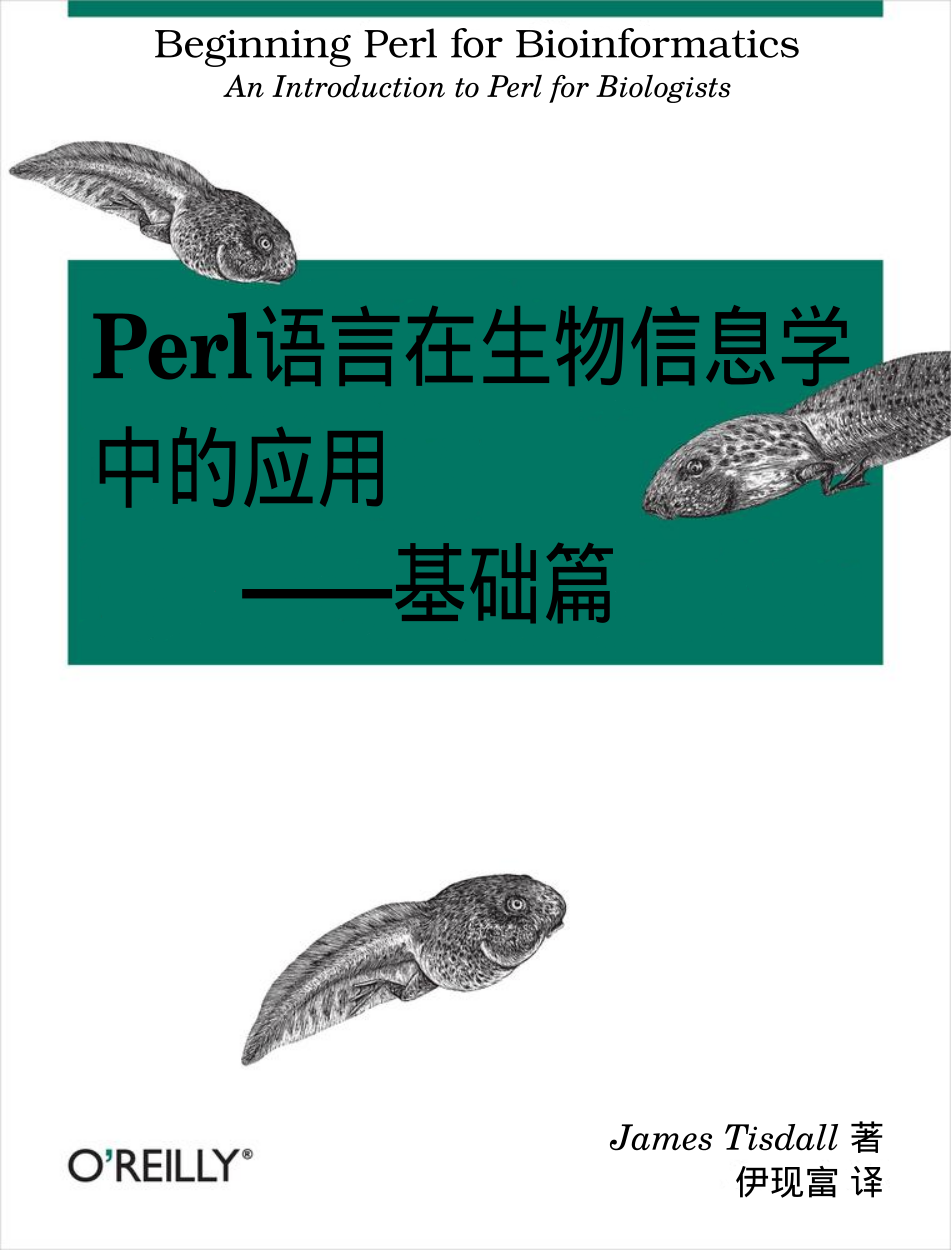
\includegraphics[width=6cm]{c1_intro_textbook.png}
  \end{figure}
\end{frame}

\begin{frame}
  \frametitle{课程安排 | 理论课}
  \begin{center}
  \alert{前9周,每周三/五,\\ 上午后两节(10:00-11:40)/下午前两节(13:30-15:10),\\ 西楼501/510}\\
  \vspace{0.2cm}
  \end{center}
  \begin{block}{授课内容}
    \begin{itemize}
      \item 教材内容:第一章……~第十章
      \item 补充知识:Markdown, Git, ...
    \end{itemize}
  \end{block}
\end{frame}

\begin{frame}
  \frametitle{课程安排 | 理论课 | 自主学习}
  \begin{itemize}
    \item 上课期间以小组形式(建议以宿舍为单位)编写程序
    \item 任务主题不限(兴趣主导,生信方面的最好)
    \item 理论课的最后一/两次课(2~4学时)进行报告
    \item 小组成员人人都要参与
    \item 既参与编程又进行报告者加分
    \item 作为平时成绩的一大部分
  \end{itemize}
\end{frame}

\begin{frame}
  \frametitle{课程安排 | 理论课 | 自主学习 | 实例}
  \begin{block}{目的}
    按照用户的需求生成随机密码。
  \end{block}
  \pause
  \begin{block}{需求}
    \begin{itemize}
      \item 指定生成密码的元素(默认:混合使用数字、大小写字母、符号)
      \item 指定生成密码的长度(默认:12个字符)
      \item 指定生成密码的个数(默认:1个)
      \item 指定密码中元素的比例/字符数(默认:无比例/字符数要求)
      \item 指定需要排除的元素(比如:0和O,1和l;默认:无)
      \item 挖掘更多人性化需求……
    \end{itemize}
  \end{block}
  \pause
  \begin{block}{代码仓库}
    \begin{itemize}
      \item \href{https://github.com/Yixf-Education/project_Perl}{Yixf-Education/project\_Perl}
    \end{itemize}
  \end{block}
\end{frame}

\begin{frame}
  \frametitle{课程安排 | 实验课}
  \begin{center}
  \alert{前9周,每周三,下午前两节(13:30-15:10),教一楼304}\\
  \vspace{0.2cm}
  \end{center}
  \begin{block}{实验内容}
    \begin{itemize}
      \item 紧跟理论课进度
      \item 幻灯片与教材上的程序/实例
    \end{itemize}
  \end{block}
\end{frame}

\begin{frame}
  \frametitle{课程安排 | 考核方式}
  \begin{enumerate}
    \item 理论课:80\%
      \begin{enumerate}
        \item 平时表现:5\%
        \item 课堂测验:5\%(期中)+5\%(期末)
        \item 自主学习:15\%
        \item 闭卷考试:50\%
      \end{enumerate}
    \item 实验课:20\%
      \begin{enumerate}
        \item 平时表现:10\%
        \item 实验报告:10\%
      \end{enumerate}
  \end{enumerate}
\end{frame}



\section{生物信息学}
\begin{frame}
  \frametitle{生物信息学(bioinformatics)}
  \begin{quotation}
    ``If you can't do bioinformatics, you can't do biology."
    \begin{flushright}
    Lincoln Stein (Biologist and former CSHL Professor)
  \end{flushright}
  \end{quotation}
  \vspace{-1em}
  \begin{figure}
    \centering
    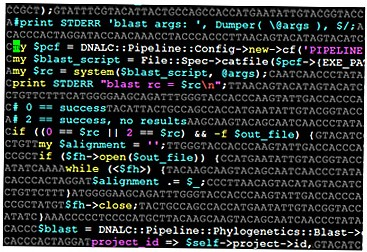
\includegraphics[width=8cm]{c1_intro_code.jpg}
  \end{figure}
  \vspace{-1em}
  Nothing in Biology Makes Sense Except in the Light of Evolution\\ \textcolor{gray}{and Bioinformatics}.
\end{frame}

\begin{frame}
  \frametitle{生物信息学 | 维基百科}
生物信息学(bioinformatics)利用应用数学、信息学、统计学和计算机科学的方法研究生物学的问题。\\
  \vspace{1em}
生物信息学的\alert{研究材料和结果}就是各种各样的生物学数据,其\alert{研究工具}是计算机,\alert{研究方法}包括对生物学数据的搜索(收集和筛选)、处理(编辑、整理、管理和显示)及利用(计算、模拟)。\\
  \vspace{1em}
  目前主要的研究方向有:序列比对、序列组装、基因识别、基因重组、蛋白质结构预测、基因表达、蛋白质反应的预测,以及建立进化模型。\\
\end{frame}

\begin{frame}
  \frametitle{生物信息学 | 维基百科(续)}
生物学技术往往生成大量的嘈杂数据。与数据挖掘类似,生物信息学利用数学工具从大量数据中提取有用的生物学信息。生物信息学所要处理的典型问题包括:重新组装在霰弹枪测序法测序过程中被打散的DNA序列,从蛋白质的氨基酸序列预测蛋白质结构,利用mRNA微阵列或质谱仪的数据检验基因调控的假说。\\
  \vspace{1em}
某些人将计算生物学作为生物信息学的同义词处理;但是另外一些人认为计算生物学和生物信息学应当被当作不同的条目处理,因为生物信息学更侧重于生物学领域中计算方法的使用和发展,而计算生物学强调应用信息学技术对生物学领域中的假说进行检验,并尝试发展新的理论。
\end{frame}

\begin{frame}
  \frametitle{生物信息学 | 维基百科(续)}
  生物信息学可以定义为对分子生物学中两类信息流的研究:\\
  \vspace{1em}
第一类信息流源于分子生物学的中心法则:DNA序列被转录为mRNA序列,后者被翻译为蛋白质序列。蛋白质序列继而折叠为具有功能的三维结构。按照达尔文演化理论,这些功能被生物体的环境所选择,从而驱动群体中DNA序列的进化。因此,第一类的生物信息学应用关注于中心法则中任一阶段的信息传递,包括DNA序列中基因的组织与控制、确定DNA中的转录单位、从序列预测蛋白质结构以及分子功能分析。\\
  \vspace{1em}
第二类信息流是基于科学方法:提出关于生物学活动的假设,设计实验以验证这些假设,评估结果与假设的相容性,然后根据实验数据对原假设作扩展或修正。第二类的生物信息学应用关注于这一流程中的信息传递,包括产生假设、设计实验、通过数据库将实验结果组织起来、检验数据与模型的相容性以及修正假设的各个系统。
\end{frame}

\begin{frame}
  \frametitle{生物信息学 | 是什么? | 学科角度}
  \begin{figure}
    \centering
    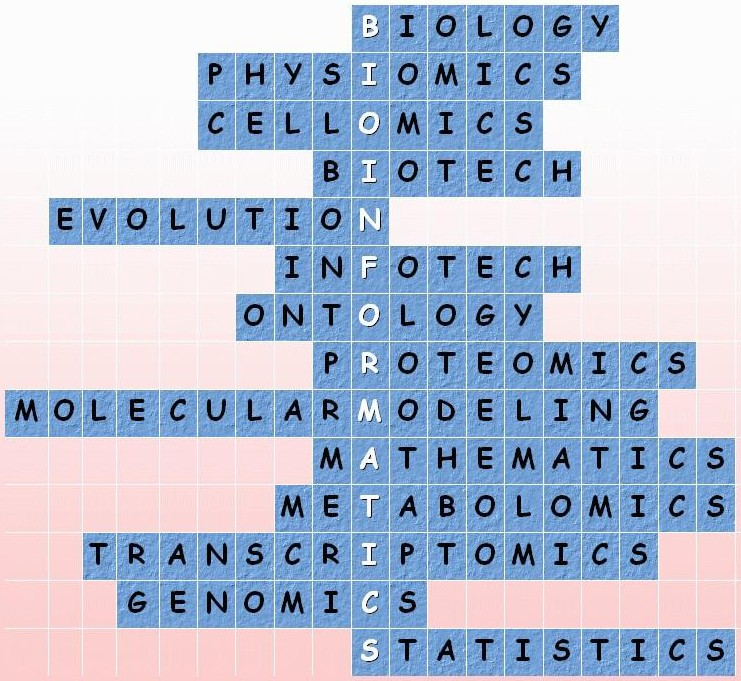
\includegraphics[width=10.5cm,height=7.5cm]{c1_intro_bioinfo_what_01.jpg}
  \end{figure}
\end{frame}

\begin{frame}
  \frametitle{生物信息学 | 是什么? | 学科角度}
  \begin{figure}
    \centering
    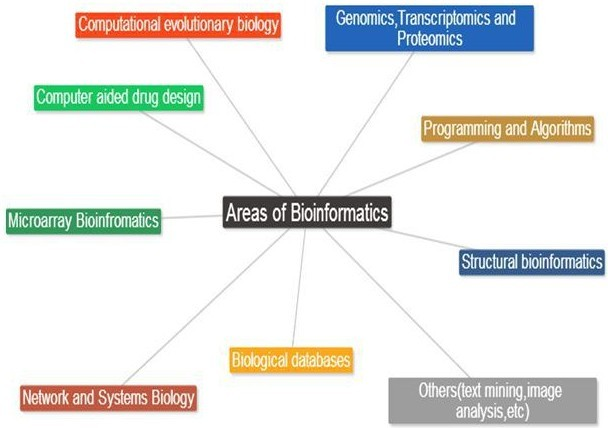
\includegraphics[width=10cm]{c1_intro_bioinfo_what_02.jpg}
  \end{figure}
\end{frame}

\begin{frame}
  \frametitle{生物信息学 | 是什么? | \alert{学科角度}}
  \begin{figure}
    \centering
    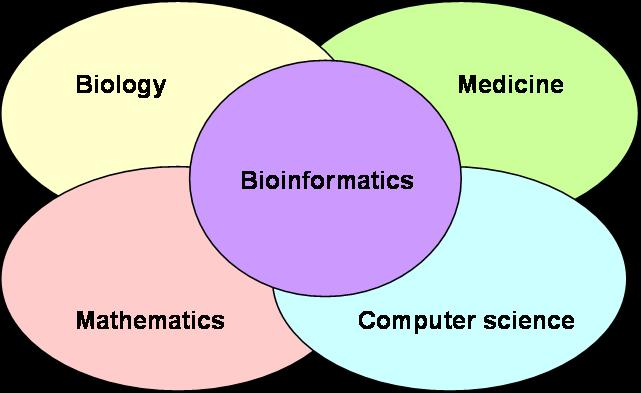
\includegraphics[width=10cm]{c1_intro_bioinfo_what_03.jpg}
  \end{figure}
\end{frame}

\begin{frame}
  \frametitle{生物信息学 | 是什么? | \alert{技术角度}}
  \begin{figure}
    \centering
    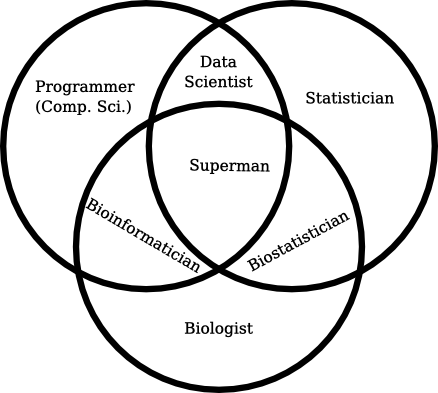
\includegraphics[width=8.5cm]{c1_intro_bioinfo_what_04.png}
  \end{figure}
\end{frame}

\begin{frame}
  \frametitle{生物信息学 | \alert{做什么?}}
  \begin{figure}
    \centering
    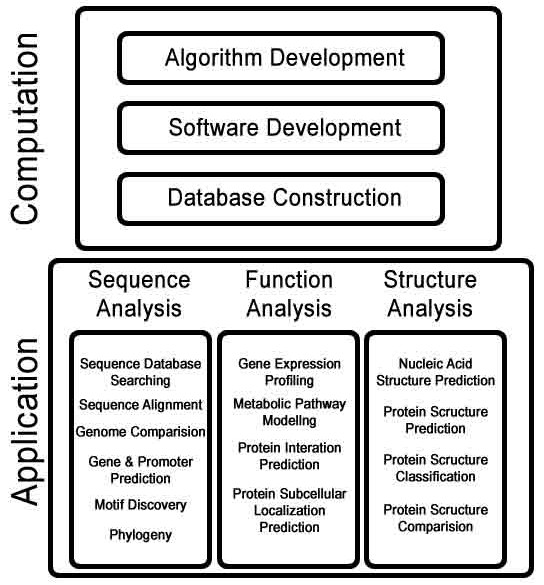
\includegraphics[width=7cm]{c1_intro_bioinfo_do.jpg}
  \end{figure}
\end{frame}

\begin{frame}
  \frametitle{生物信息学 | 资源(数据库与工具)}
  \begin{figure}
    \centering
    
\includegraphics[width=10.5cm]{c1_intro_bioinfo_resource.png}
  \end{figure}
\end{frame}

\begin{frame}
  \frametitle{生物信息学 | 资源(技术与工具)}
  \begin{figure}
    \centering
    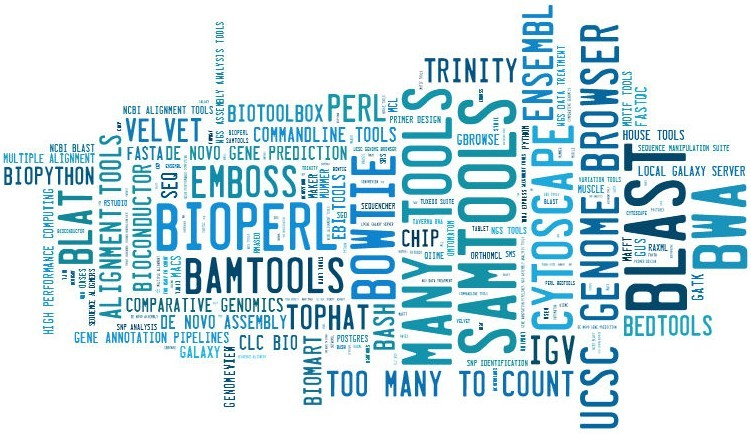
\includegraphics[width=11cm]{c1_intro_bioinfo_tool_01.jpg}
  \end{figure}
\end{frame}

\begin{frame}
  \frametitle{生物信息学 | 主题词}
  \begin{figure}
    \centering
    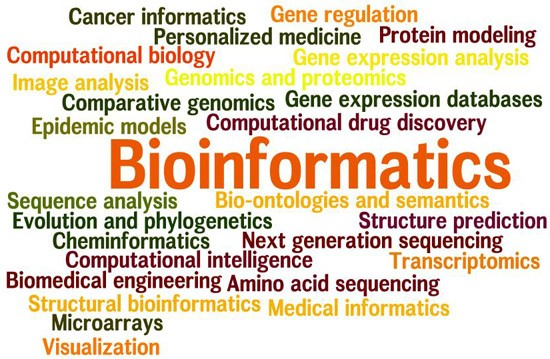
\includegraphics[width=10.5cm]{c1_intro_bioinfo_topic_01.jpg}
  \end{figure}
\end{frame}

\begin{frame}
  \frametitle{生物信息学 | 主题词}
  \begin{figure}
    \centering
    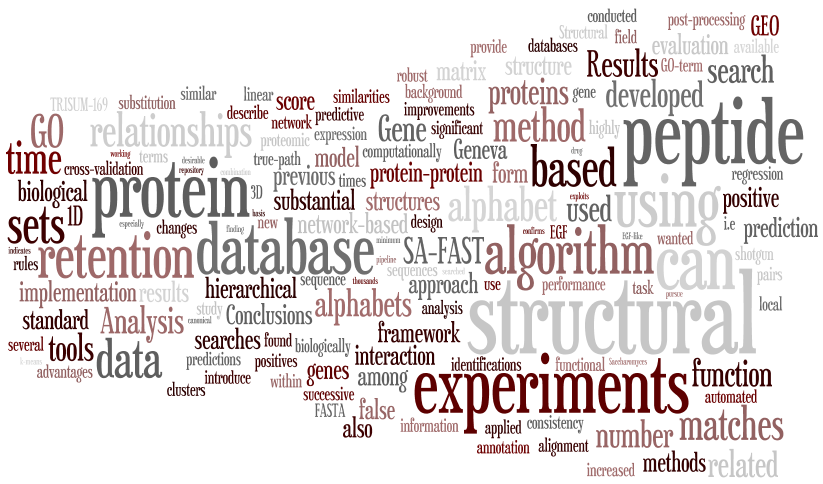
\includegraphics[width=10.5cm]{c1_intro_bioinfo_topic_02.png}
  \end{figure}
\end{frame}

\begin{frame}
  \frametitle{生物信息学 | 总结}
  \begin{center}
    {\Large 生物信息学家 = 生命科学中的黑客!}
  \end{center}
  \vspace{-1em}
  \begin{figure}
    \centering
    
\includegraphics[width=9cm]{c1_intro_bioinfo_matrix.png}
  \end{figure}
\end{frame}

\section{生物学}
\begin{frame}
  \frametitle{生物学 | 历史}
  \begin{figure}
    \centering
    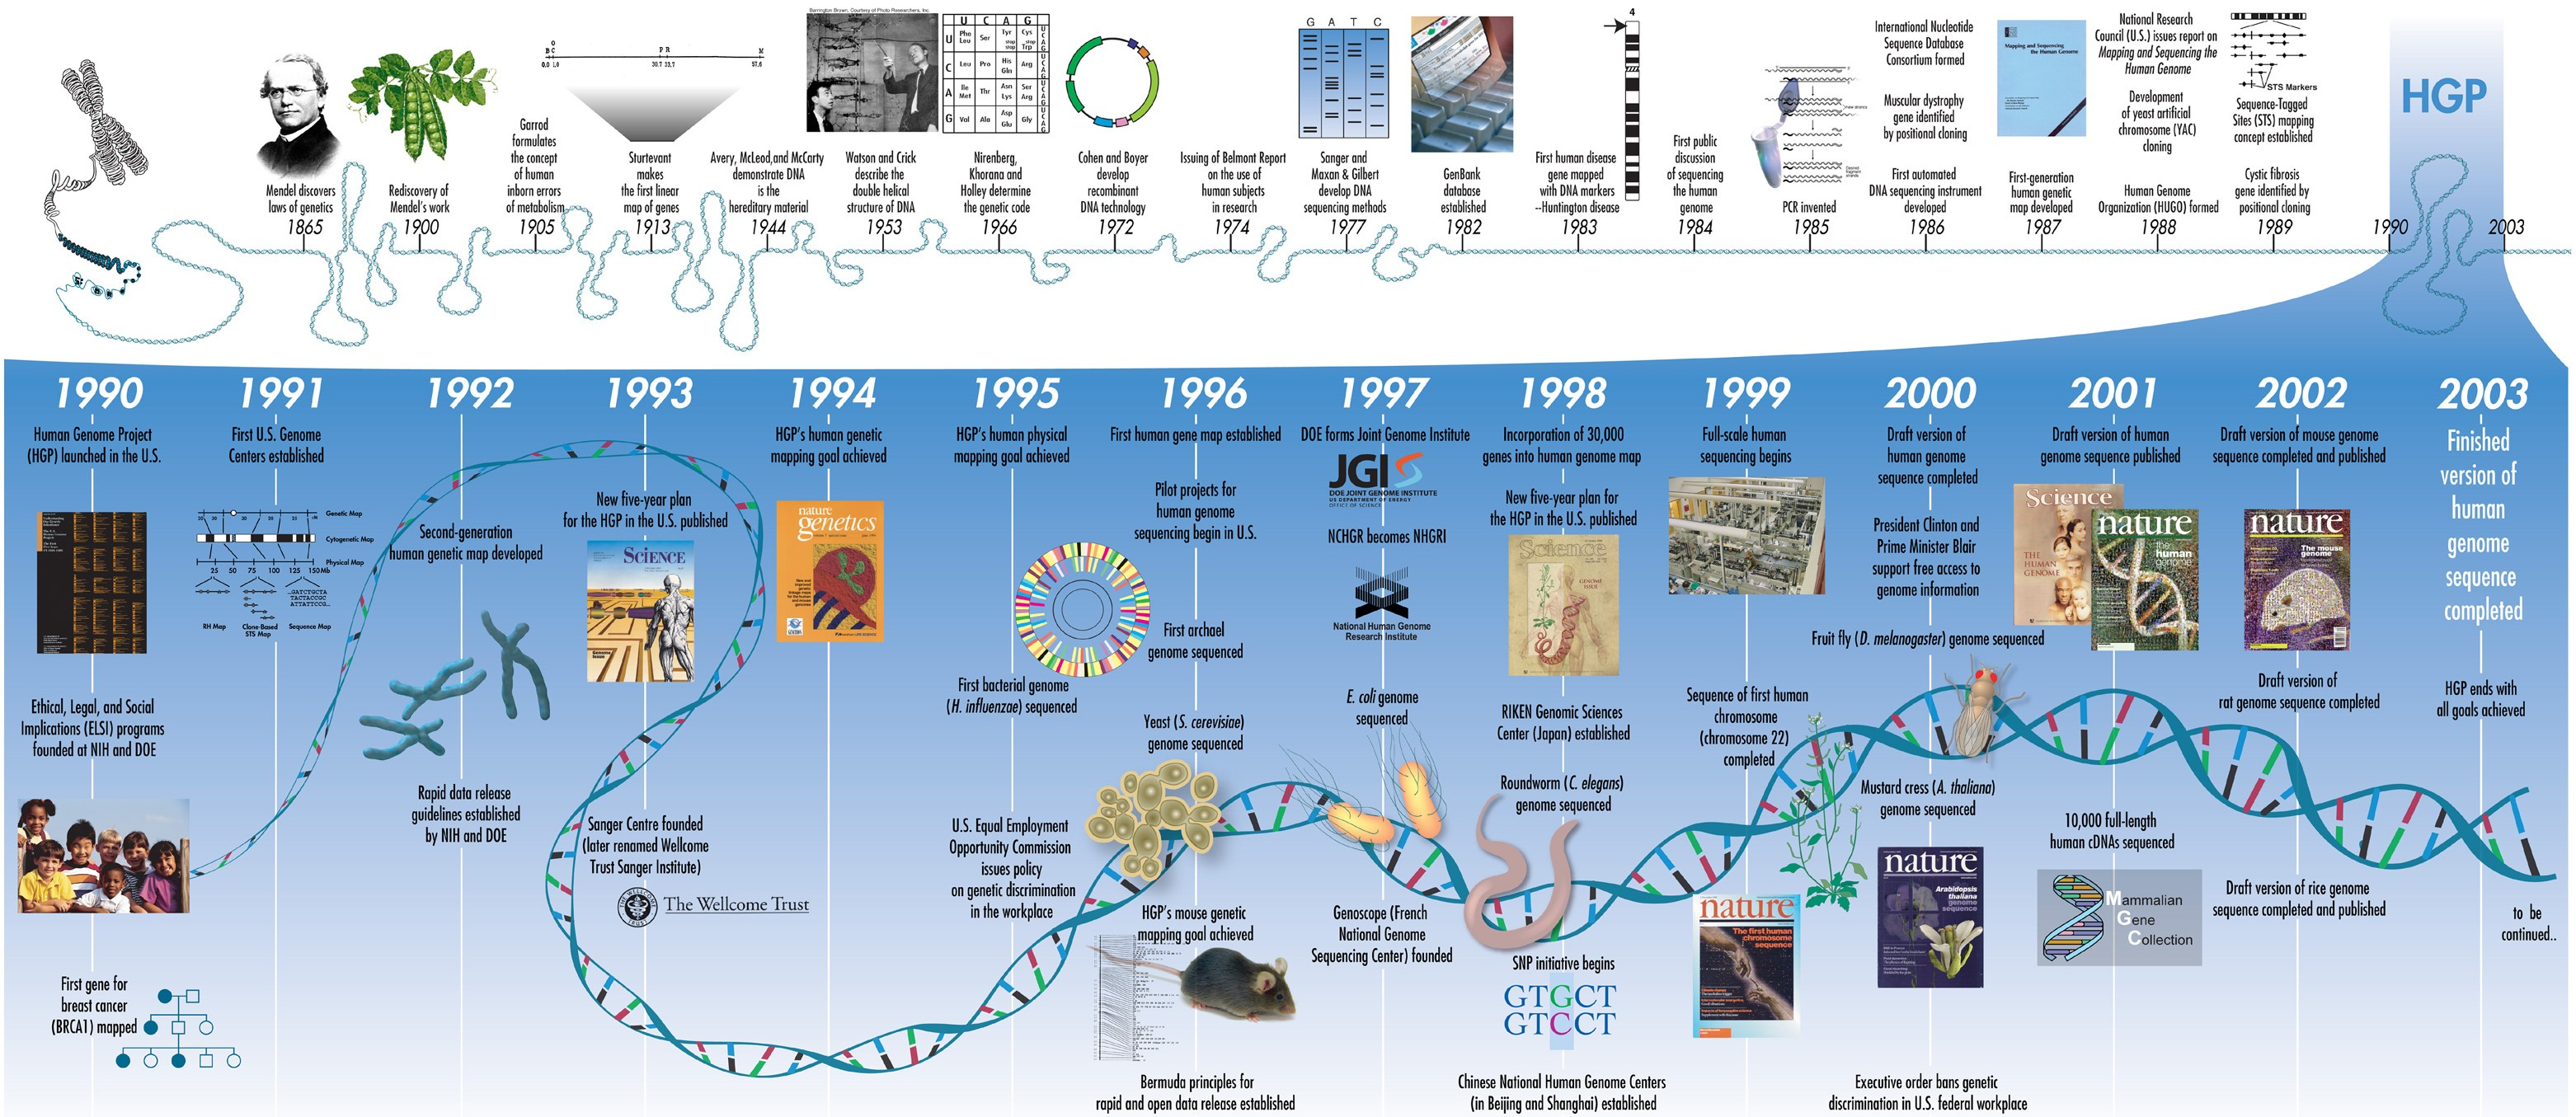
\includegraphics[width=12cm]{c1_intro_biology_history_01.jpg}
  \end{figure}
\end{frame}

\begin{frame}
  \frametitle{生物学 | 中心法则(central dogma)}
  \begin{figure}
    \centering
    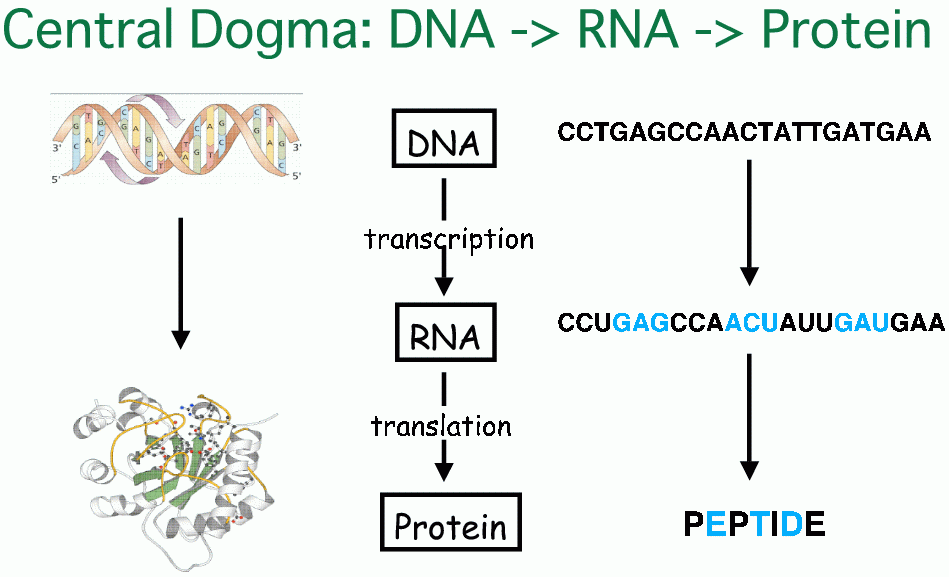
\includegraphics[width=10.5cm]{c1_intro_dogma_01.png}
  \end{figure}
\end{frame}

\begin{frame}
  \frametitle{生物学 | \alert{DNA}}
  \begin{figure}
    \centering
    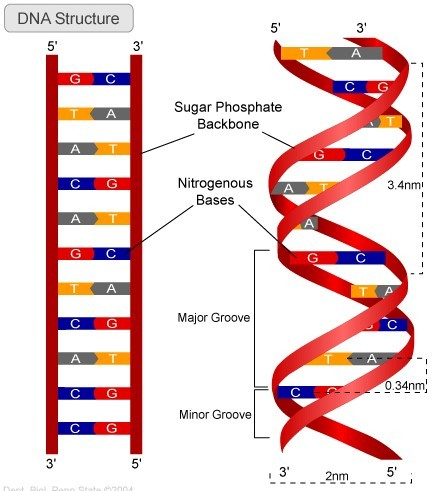
\includegraphics[width=7cm]{c1_intro_dna_01.jpg}
  \end{figure}
\end{frame}

\begin{frame}
  \frametitle{生物学 | \alert{RNA}}
  \begin{figure}
    \centering
    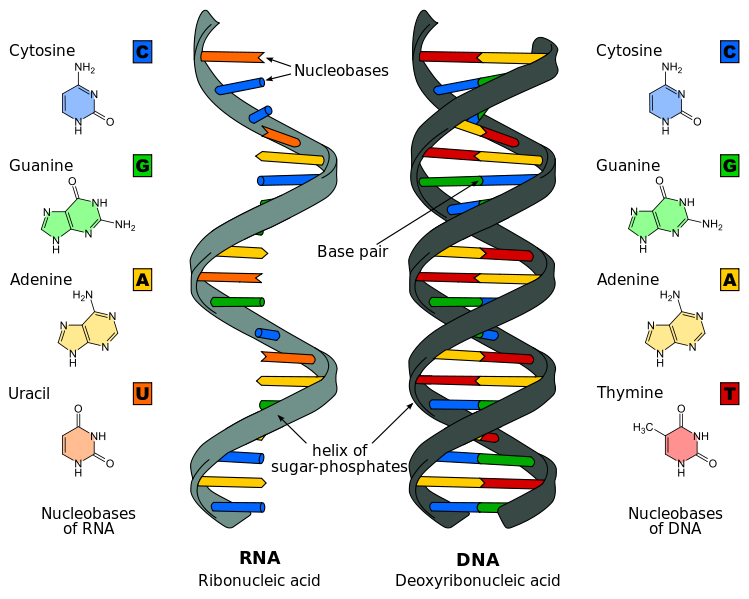
\includegraphics[width=9.5cm]{c1_intro_rna_01.png}
  \end{figure}
\end{frame}

\begin{frame}
  \frametitle{生物学 | 蛋白质 | \alert{氨基酸}}
  \vspace{-0.6em}
  \begin{figure}
    \centering
    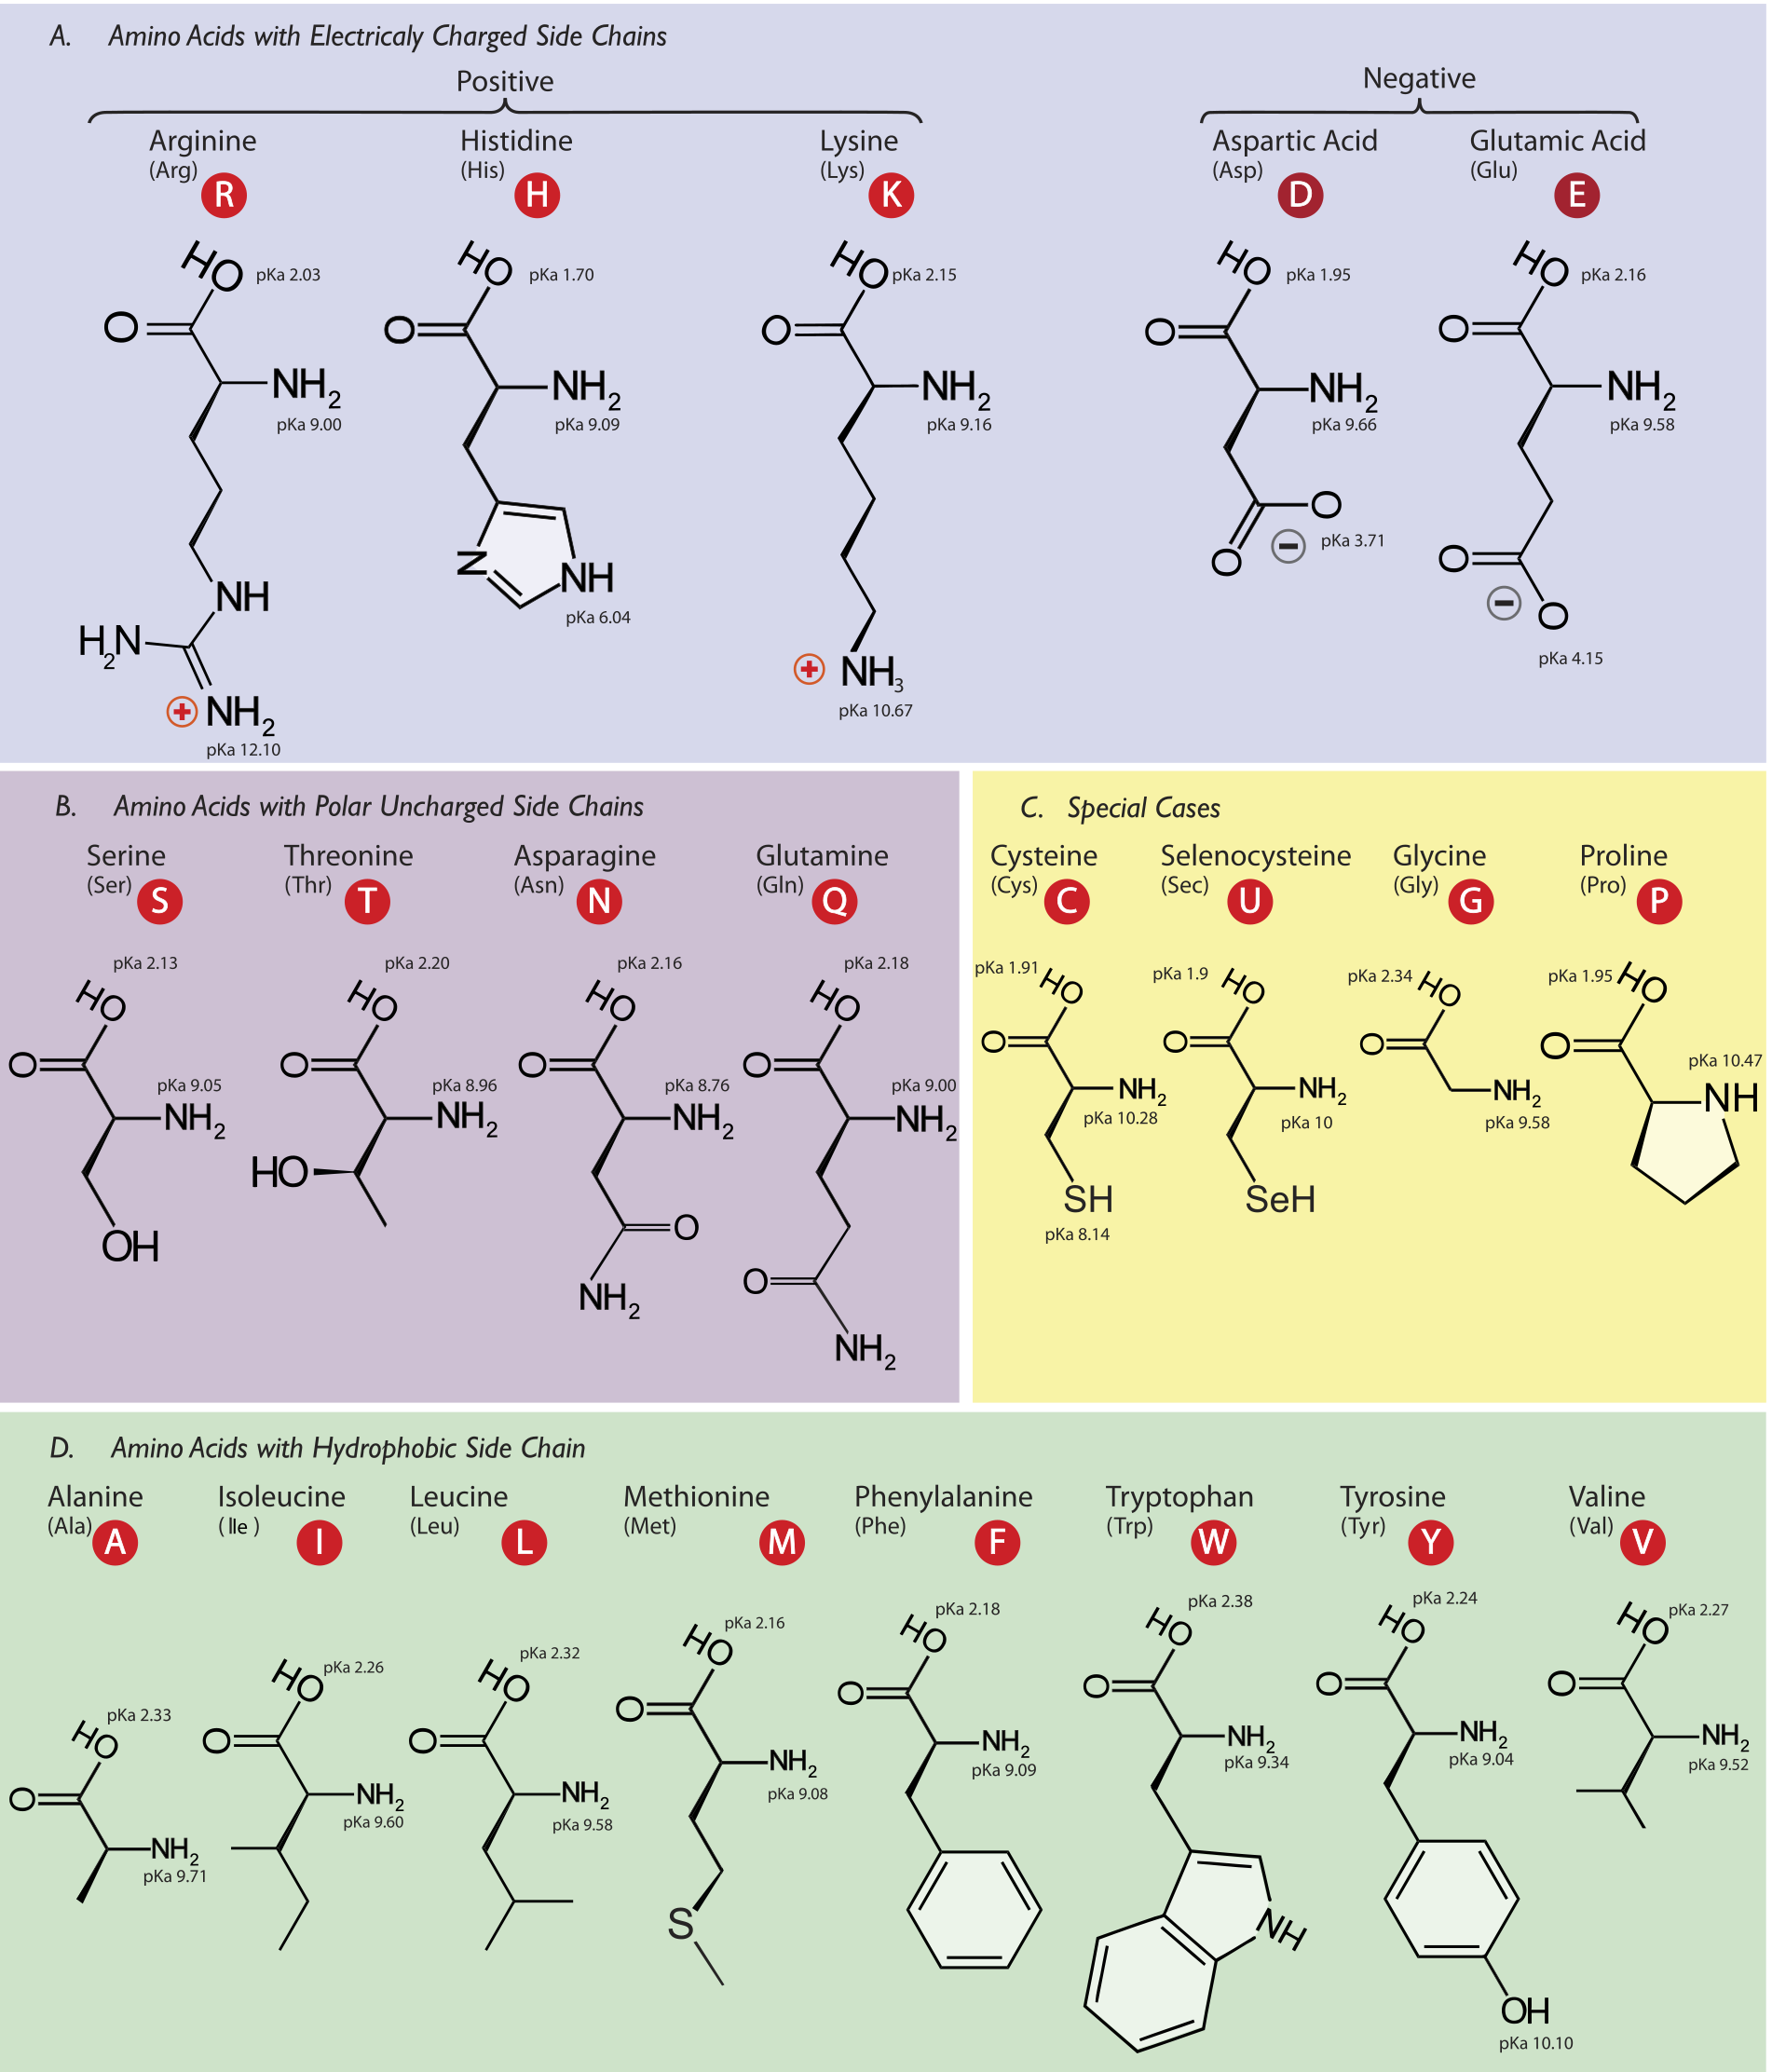
\includegraphics[width=9.5cm,height=7.8cm]{c1_intro_aa_01.png}
  \end{figure}
\end{frame}

\begin{frame}
  \frametitle{生物学 | 蛋白质 | 氨基酸 | 助记口诀}
  \begin{block}{必需氨基酸}
  甲携来一本亮色书(甲硫氨酸、缬氨酸、赖氨酸、异亮氨酸、苯丙氨酸、亮氨酸、色氨酸、苏氨酸)
\end{block}
\pause
\begin{block}{20种氨基酸}
  苏缬亮异亮,苯丙属芳香。\\
  还有色赖蛋,缺一人遭殃。\\
  (以上是必需氨基酸)\\
  丙组丝甘半,天谷建酸胺。\\
  精酪加一脯,二十氨基酸。\\
  (以上是非必需氨基酸)
\end{block}
\end{frame}

\begin{frame}
  \frametitle{生物学 | 蛋白质 | 多肽}
  \begin{figure}
    \centering
    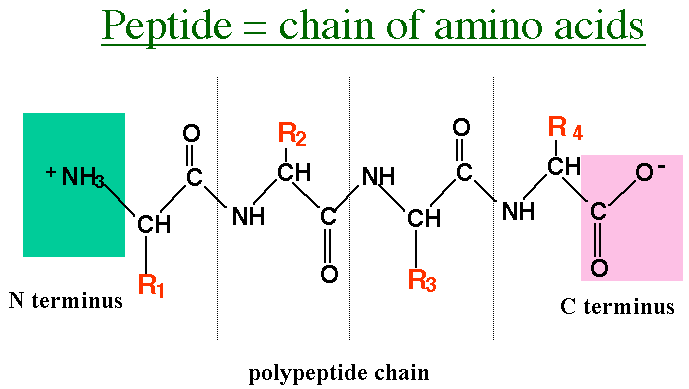
\includegraphics[width=8cm,height=3cm]{c1_intro_peptide_01.png}\\
    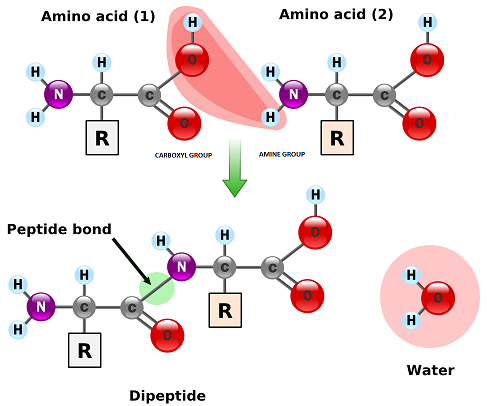
\includegraphics[width=7cm,height=4.8cm]{c1_intro_peptide_02.png}
  \end{figure}
\end{frame}

\begin{frame}
  \frametitle{生物学 | 蛋白质 | 结构}
  \begin{figure}
    \centering
    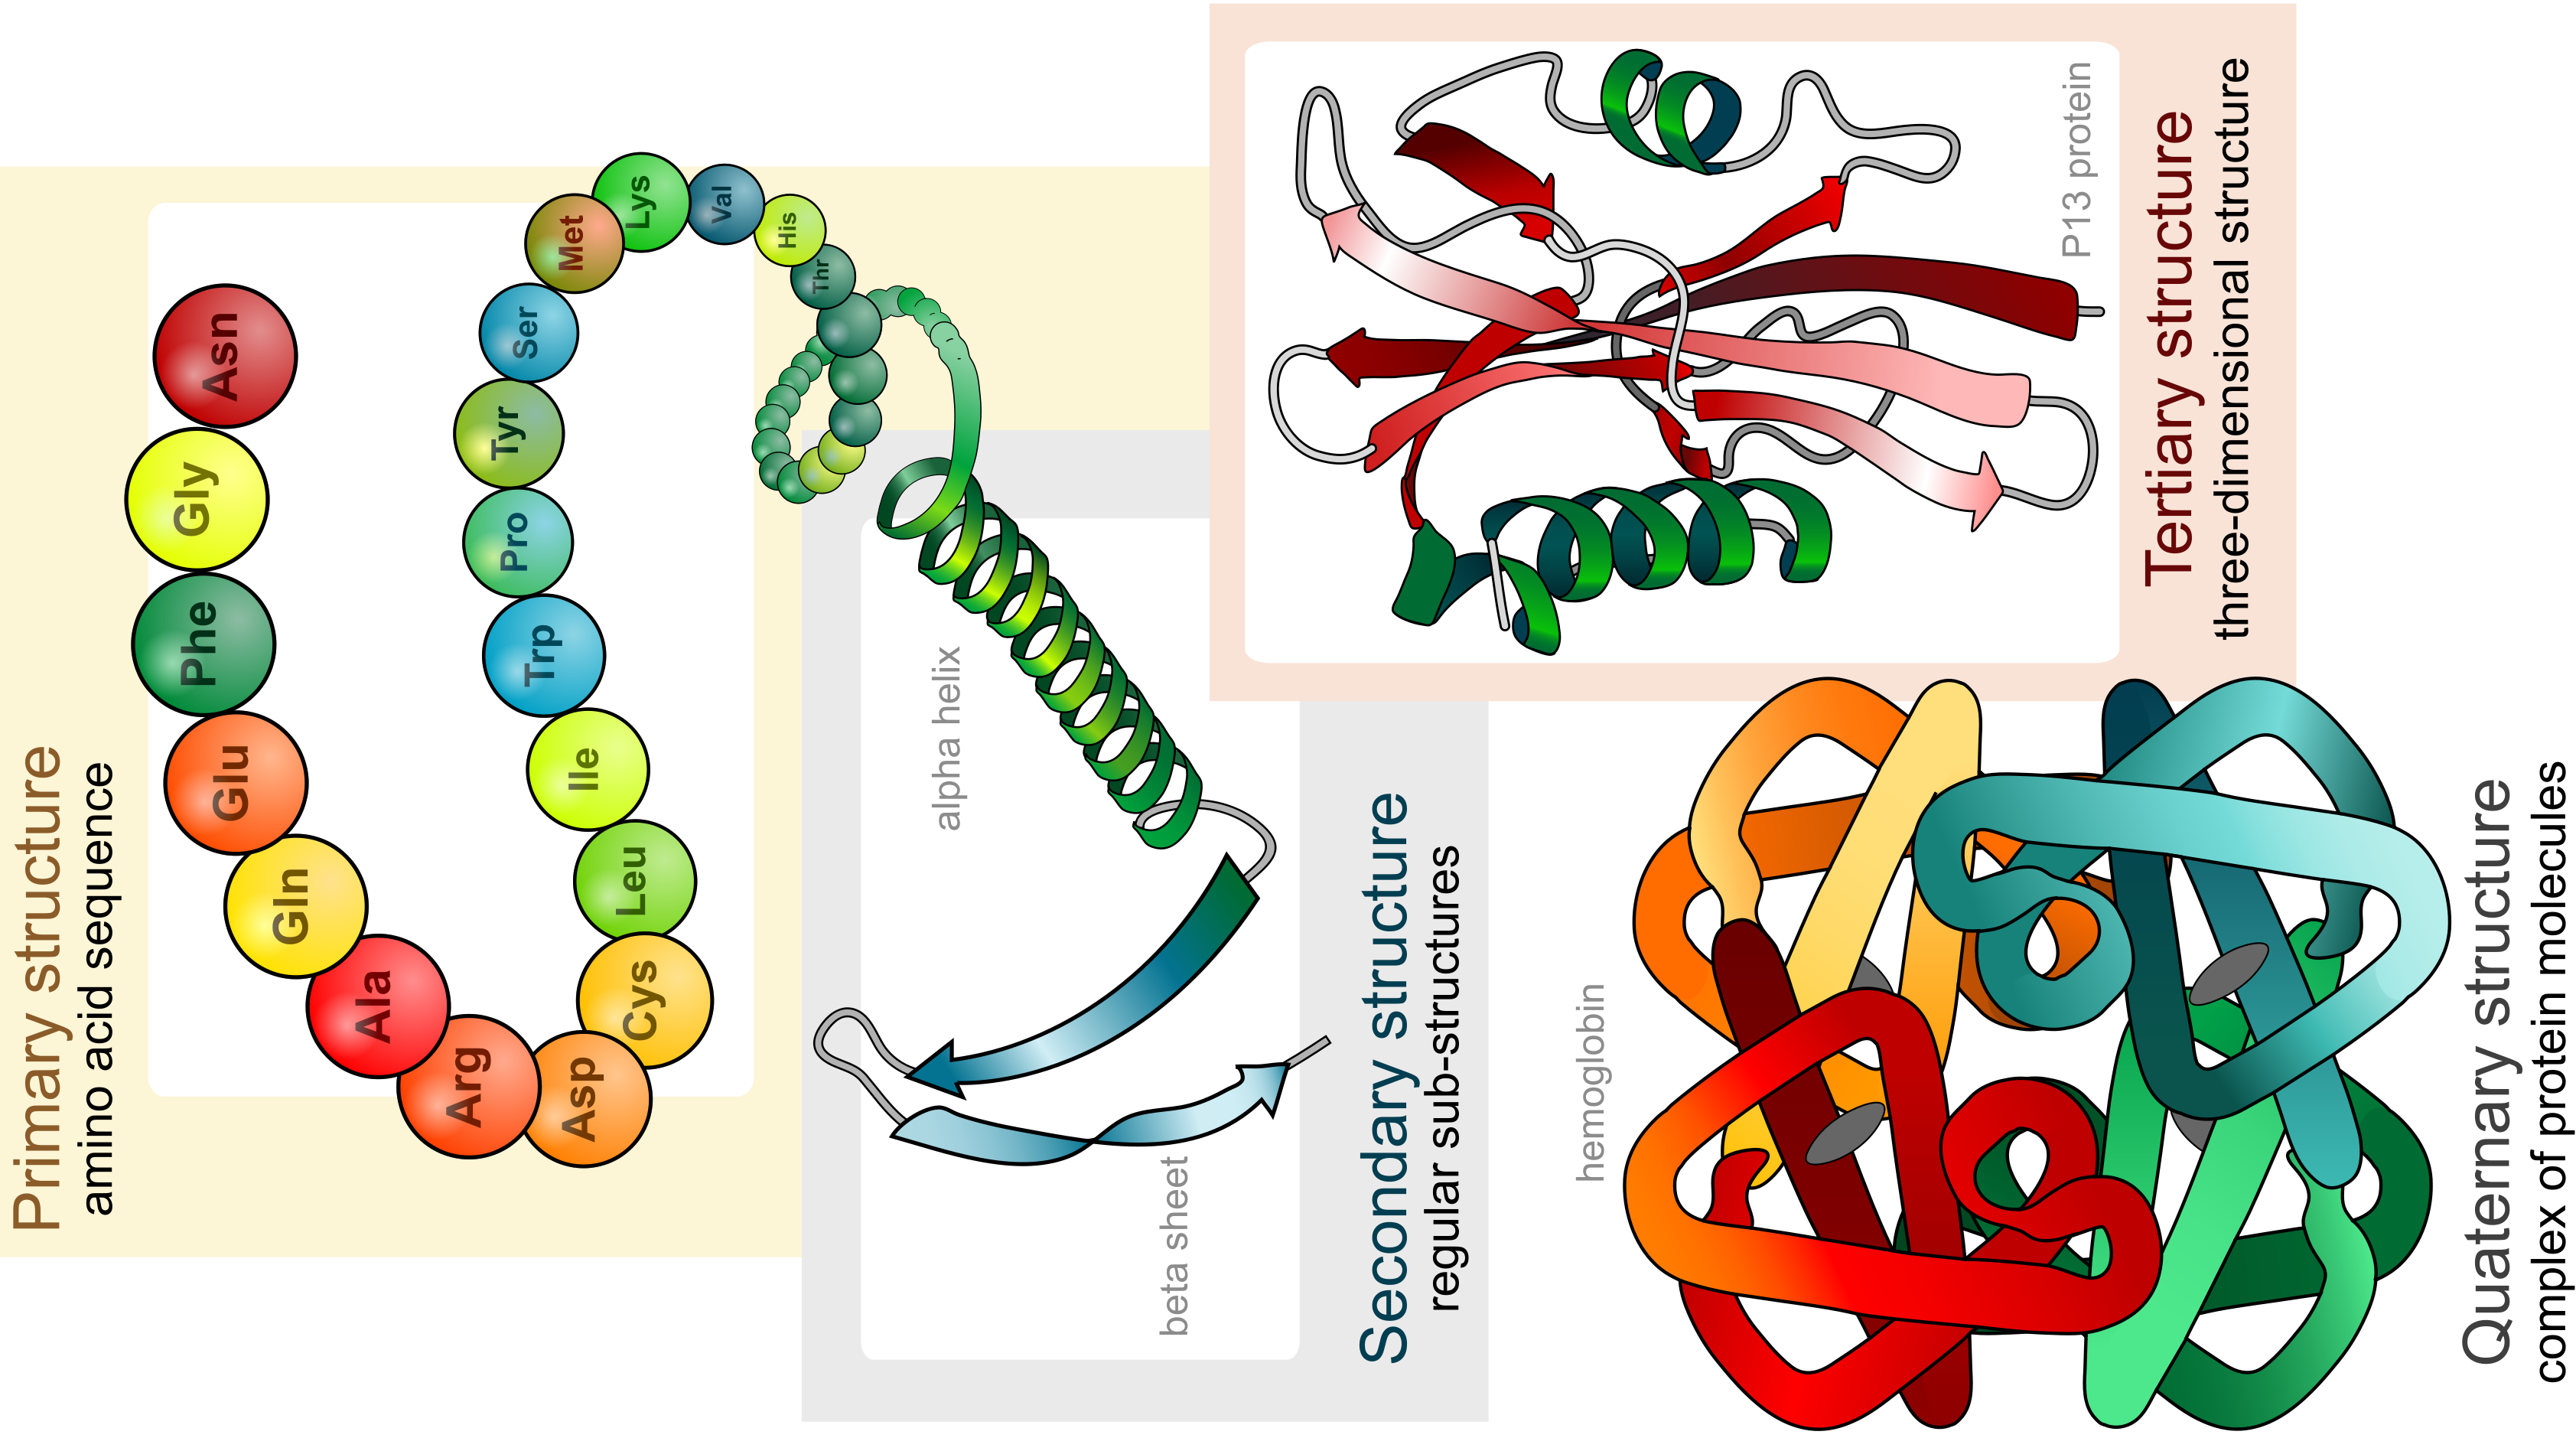
\includegraphics[width=11.5cm]{c1_intro_protein_01.png}
  \end{figure}
\end{frame}

\begin{frame}
  \frametitle{生物学 | \alert{数据库}}
  \begin{figure}
    \centering
    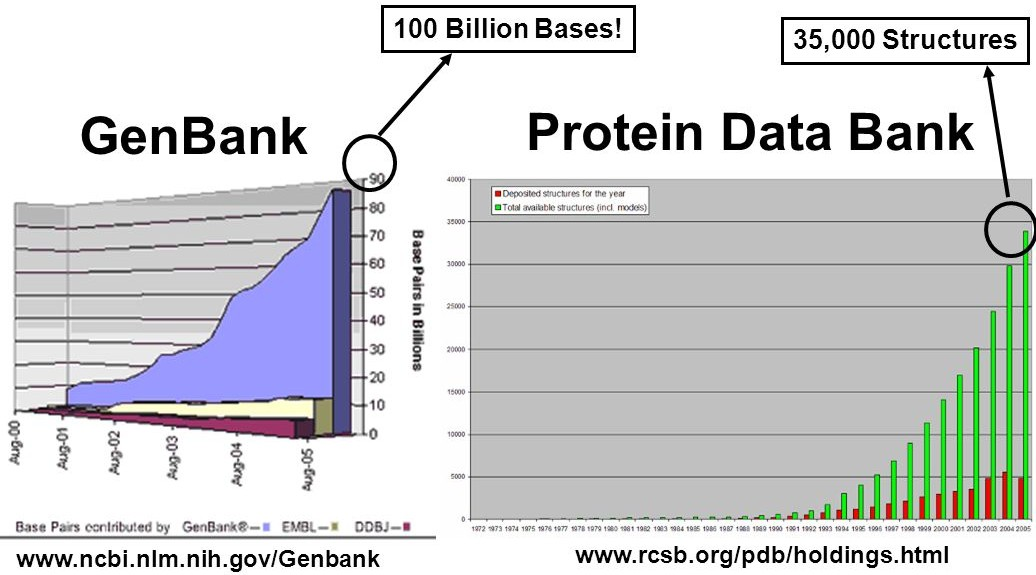
\includegraphics[width=11cm]{c1_intro_db_01.jpg}
  \end{figure}
\end{frame}

\begin{frame}
  \frametitle{生物学 | 数据库 | GenBank}
  \begin{figure}
    % \centering
    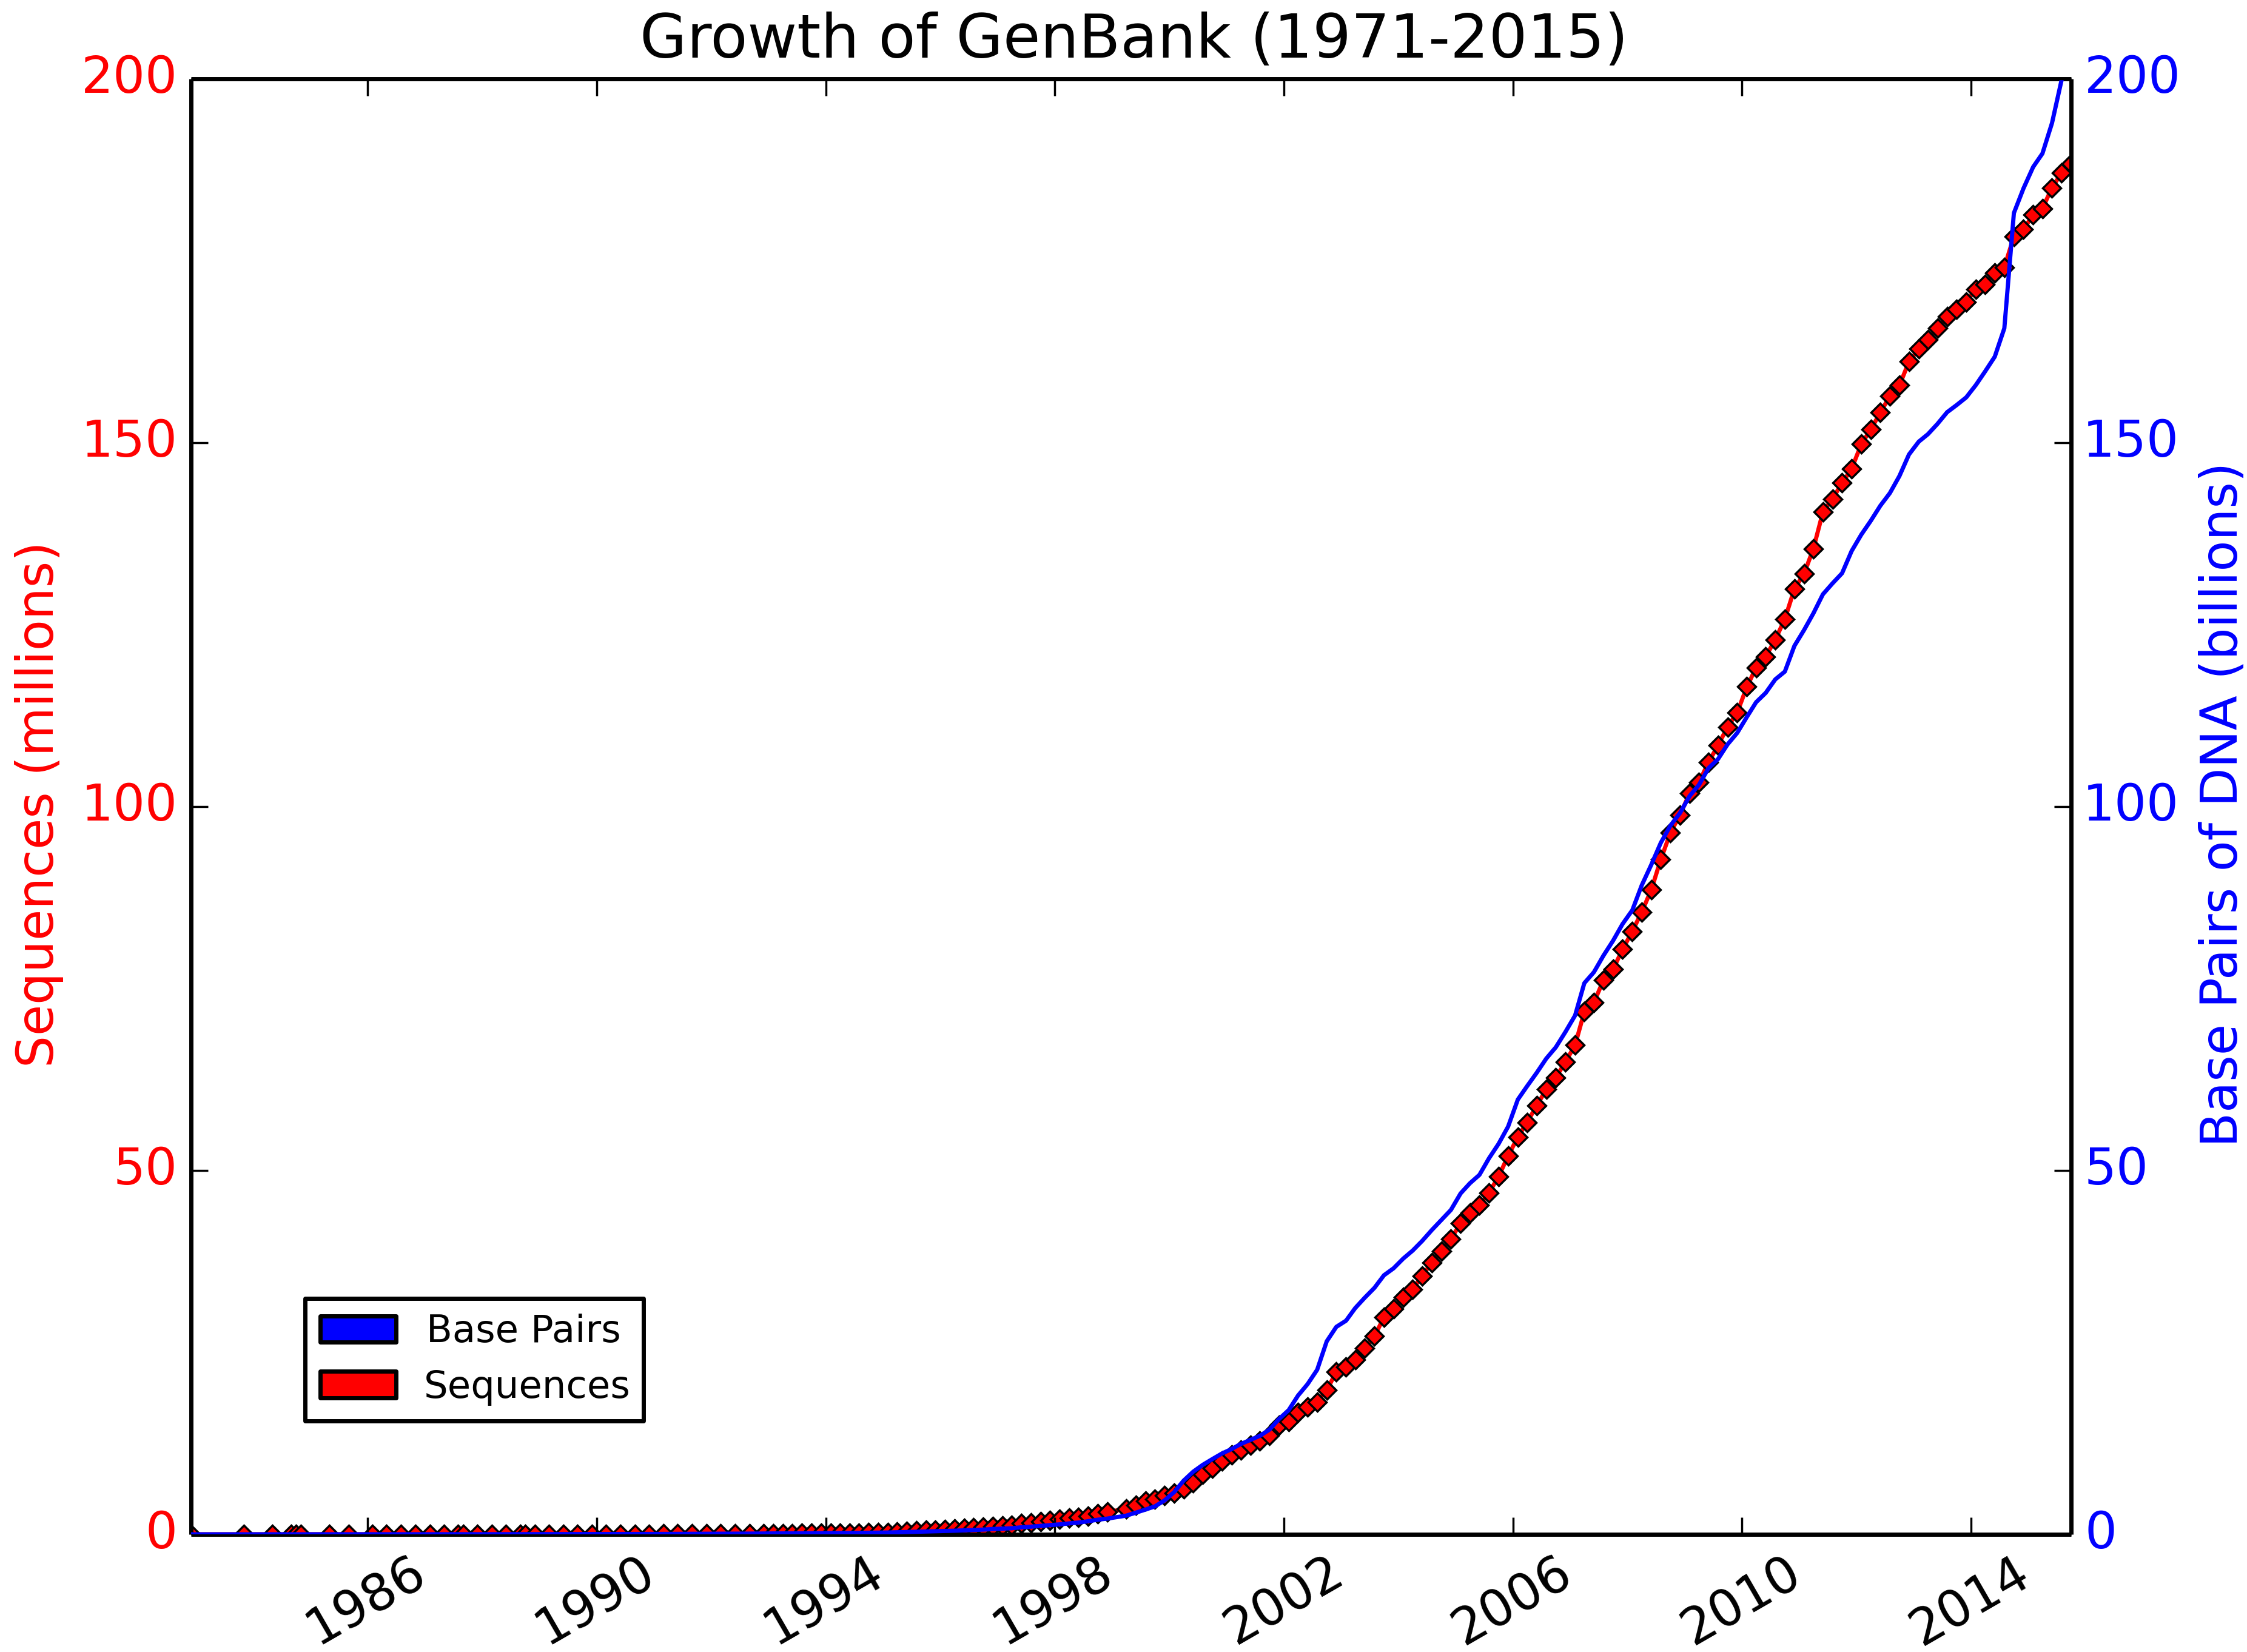
\includegraphics[width=5.5cm]{c1_intro_db_02.png}
    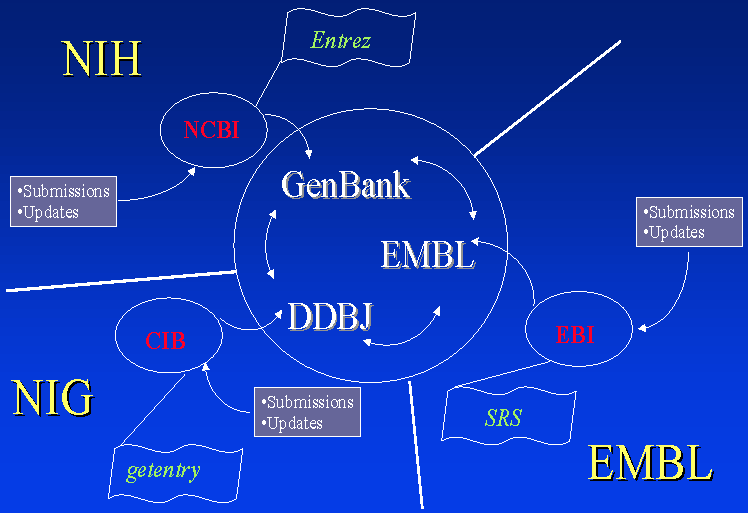
\includegraphics[width=5.8cm]{c1_intro_db_05.png}
  \end{figure}
\end{frame}

\begin{frame}
  \frametitle{生物学 | 数据库 | PDB}
  \begin{figure}
    \centering
    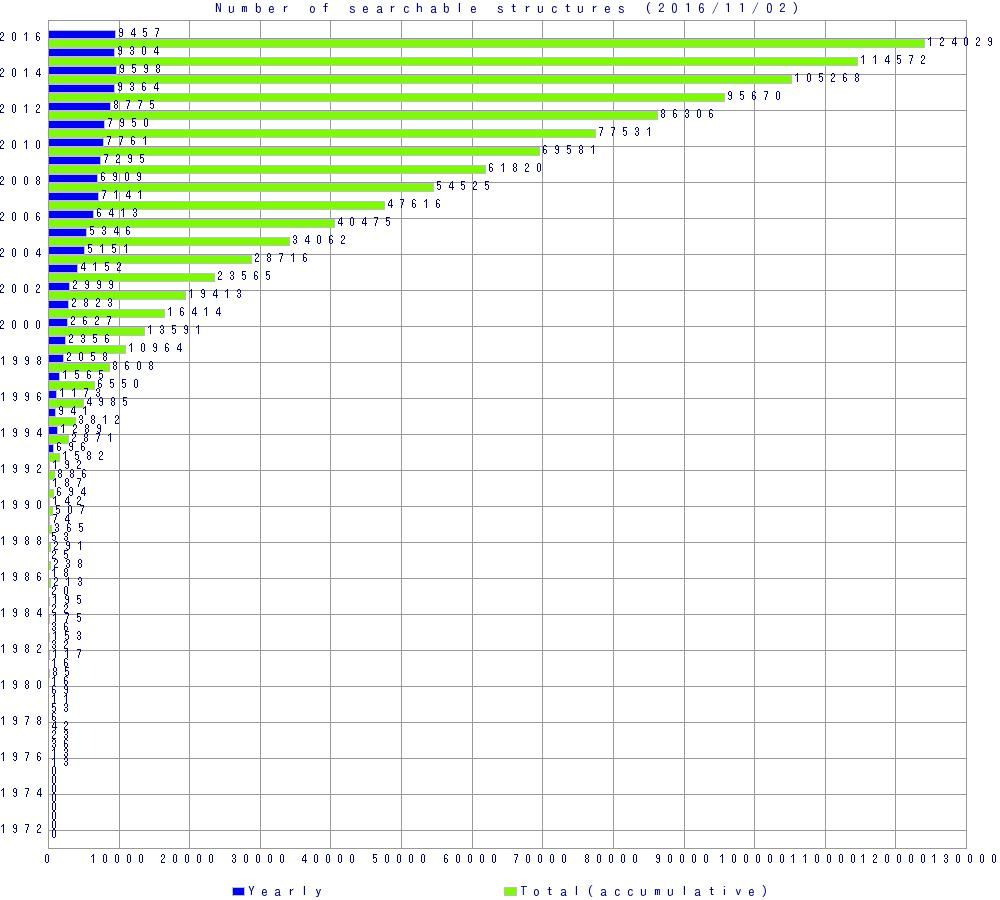
\includegraphics[width=8.5cm]{c1_intro_db_06.jpg}
  \end{figure}
\end{frame}

\begin{frame}
  \frametitle{生物学 | 数据格式}
  \begin{figure}
    \centering
    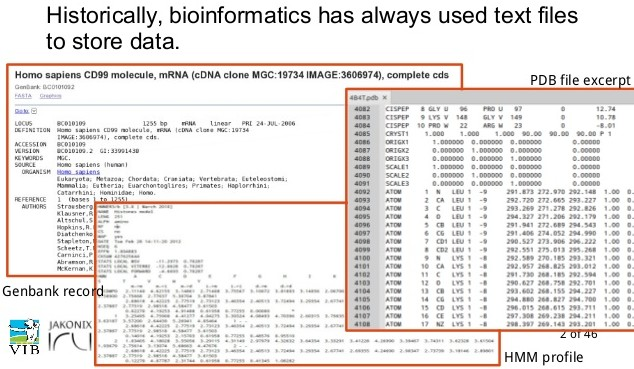
\includegraphics[width=11cm]{c1_intro_data_format_01.jpg}
  \end{figure}
\end{frame}

\section{计算机科学}
\begin{frame}
  \frametitle{计算机科学 | 历史}
  \begin{figure}
    \centering
    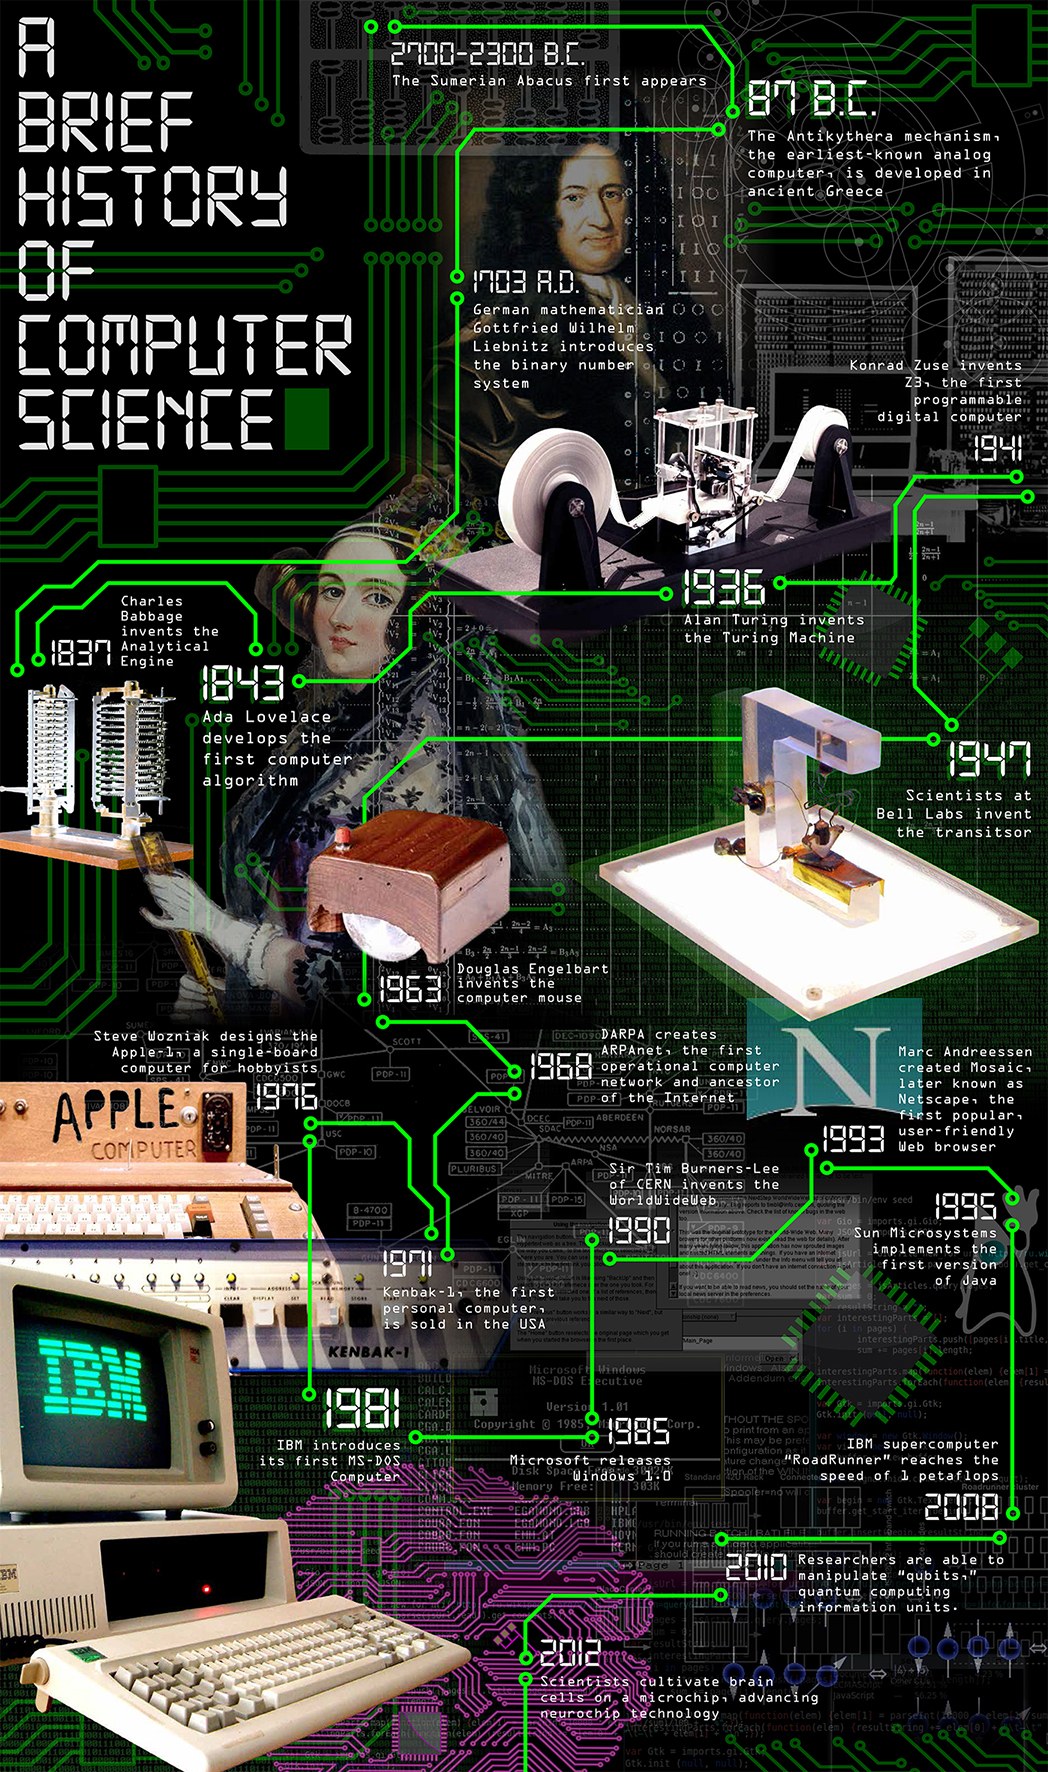
\includegraphics[width=10cm,height=7.5cm]{c1_intro_cs_history_01.png}
  \end{figure}
\end{frame}

\begin{frame}
  \frametitle{计算机科学 | \alert{术语}}
  \begin{block}{\textit{in vivo}}
  \textit{In vivo}为拉丁文“在活体内”之意。在科学文献中,\textit{in vivo}常指进行于完整且存活的个体内的组织的实验,以区别在生物体上移除下来的组织或死亡的组织上进行的实验(对应的拉丁文为\textit{in vitro })。
  \end{block}
  \pause
  \begin{block}{\textit{in vitro}}
    \textit{In vitro}是拉丁语中“在玻璃里”的意思,意指进行或发生于试管内的实验与实验技术。更广义的意思,则指活生物体之外的环境中的操作。
  \end{block}
  \pause
  \begin{block}{\textit{in silico}}
    \textit{In
    silico}是指“在硅之中”,也就是说“进行于电脑中,或是经由电脑模拟”之意,此用语是衍生自另外两个在生物学上常用的短语:\textit{in vivo}(生物活体内)及\textit{in vitro}(生物活体外)。
  \end{block}
\end{frame}

\begin{frame}
  \frametitle{计算机科学 | 编程语言}
  \begin{figure}
    \centering
    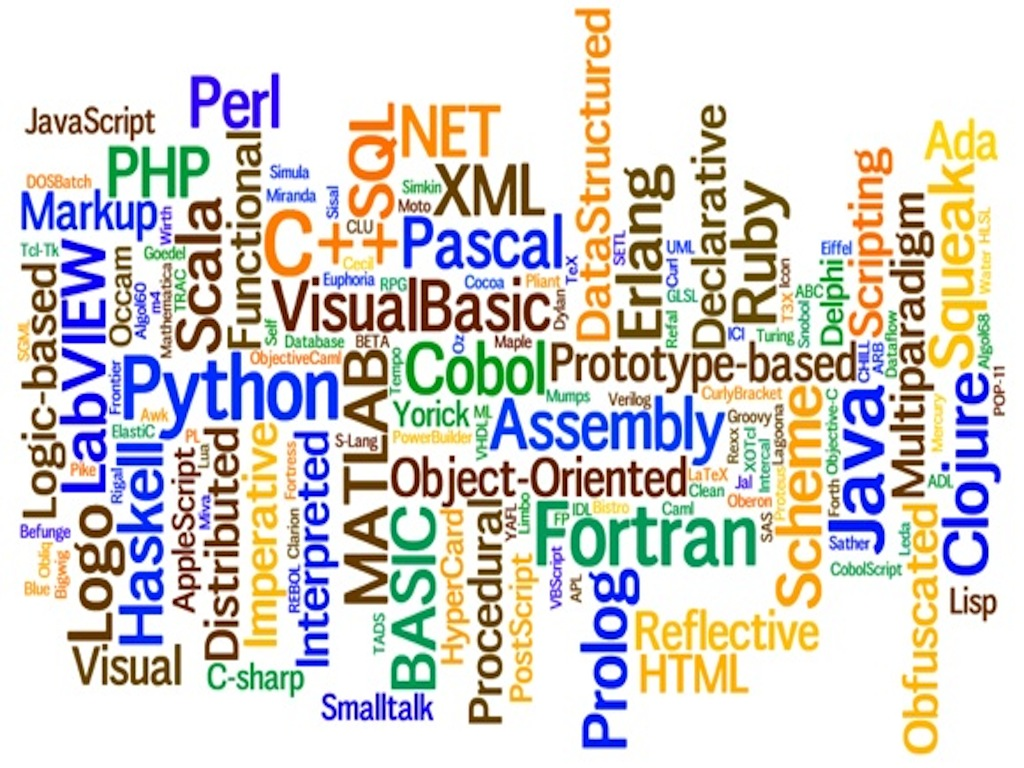
\includegraphics[width=10cm]{c1_intro_language.jpg}
  \end{figure}
\end{frame}

\begin{frame}
  \frametitle{计算机科学 | 编程语言 | 崇拜/鄙视链}
  \begin{figure}
    \centering
    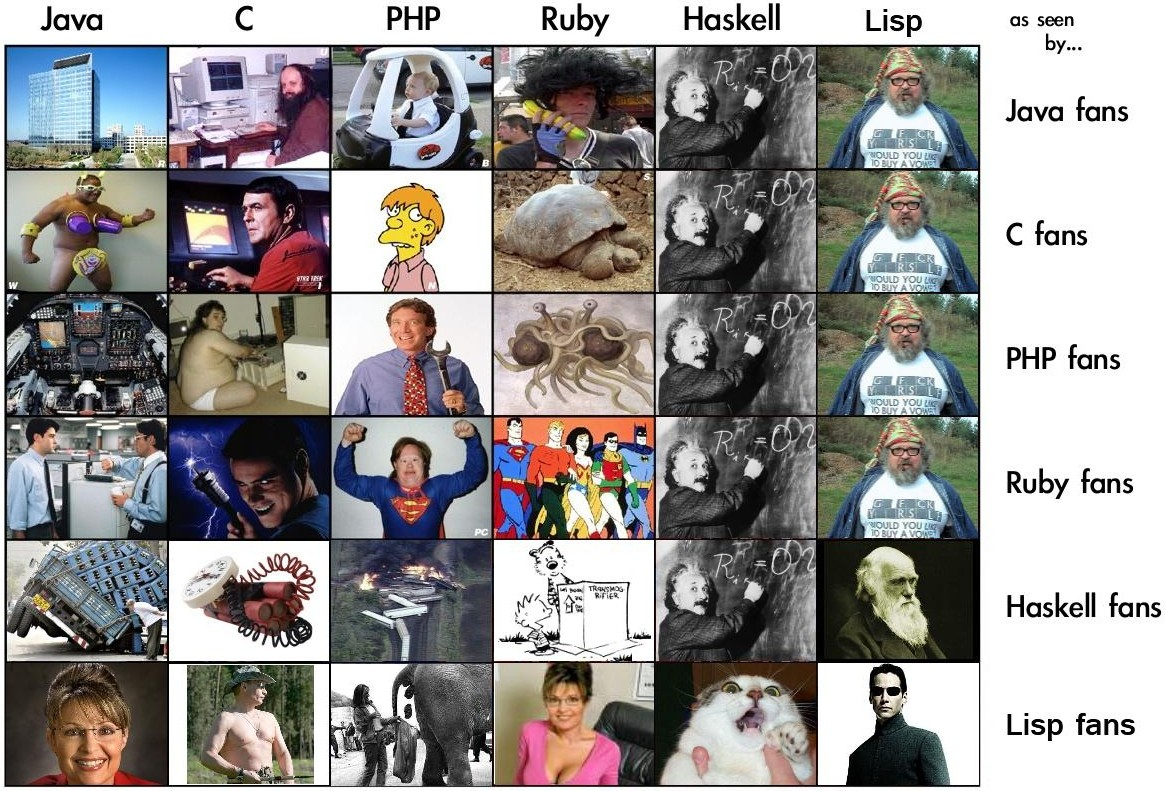
\includegraphics[width=11cm]{c1_intro_language_fanboys.jpg}
  \end{figure}
\end{frame}

\begin{frame}
  \frametitle{计算机科学 | 编程语言 | 特色}
  \begin{figure}
    \centering
    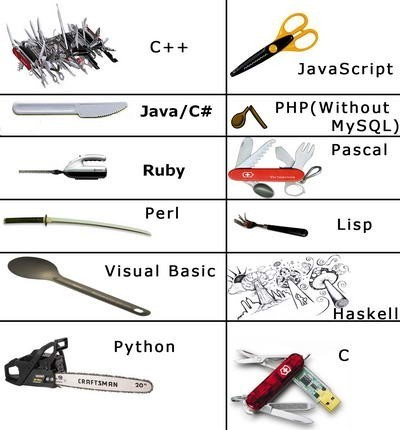
\includegraphics[width=7cm]{c1_intro_language_knife.jpg}
  \end{figure}
\end{frame}

\begin{frame}
  \frametitle{计算机科学 | 编程语言 | 如果是……}
  \begin{table}
    \centering
    \rowcolors[]{1}{blue!20}{blue!10}
    \begin{tabular}{clll}
      \hline
      \rowcolor{blue!50}语言 & 宗教 & 超级英雄 & 《哈利波特》\\
      \hline
      C & 犹太教 & --- & 伏地魔\\
      C++ & 伊斯兰教 & --- & 西弗勒斯·斯内普\\
      Java & 正统基督教 & 万磁王 & 洛雷斯·乌姆里奇\\
      Lisp & 佛教 & Xavier教授 & ---\\
      Perl & 巫毒教 & --- & 罗恩·韦斯莱\\
      PHP & Cafeteria基督教 & 小丑王 & 德拉科·马尔福\\
      Python & 人文主义 & 蝙蝠侠 & 哈利·波特\\
      Ruby & 新异教主义 & 钢铁侠 & ---\\
      shell & --- & --- & 鲁伯·海格\\
      \hline
    \end{tabular}
  \end{table}
\end{frame}

\begin{frame}
  \frametitle{计算机科学 | 编程语言 | 如果是……(续)}
  \begin{table}
    \centering
    \rowcolors[]{1}{blue!20}{blue!10}
    \begin{tabular}{clll}
      \hline
      \rowcolor{blue!50}语言 & 女人 & 武器 & 船\\
      \hline
      C & 霸道女总裁 & M1式加兰德步枪 & 核潜艇\\
      C++ & --- & 双截棍 & ---\\
      Java & 娇妻贤内助 & M240通用弹夹式自动机枪 & 大货船\\
      Lisp & 女博士 & 剃须刀 & ---\\
      Perl & --- & 燃烧弹 & 拖船\\
      PHP & --- & 水管子 & 竹筏\\
      Python & 万人迷 & 双管枪 & ---\\
      Ruby & --- & 宝刀 & 摩托艇\\
      shell & 女公务员 & 锤子 & ---\\
      \hline
    \end{tabular}
  \end{table}
\end{frame}

% reference 00_website.md to update figures
\begin{frame}
  \frametitle{计算机科学 | 编程语言 | 流行度}
  \begin{figure}
    \centering
    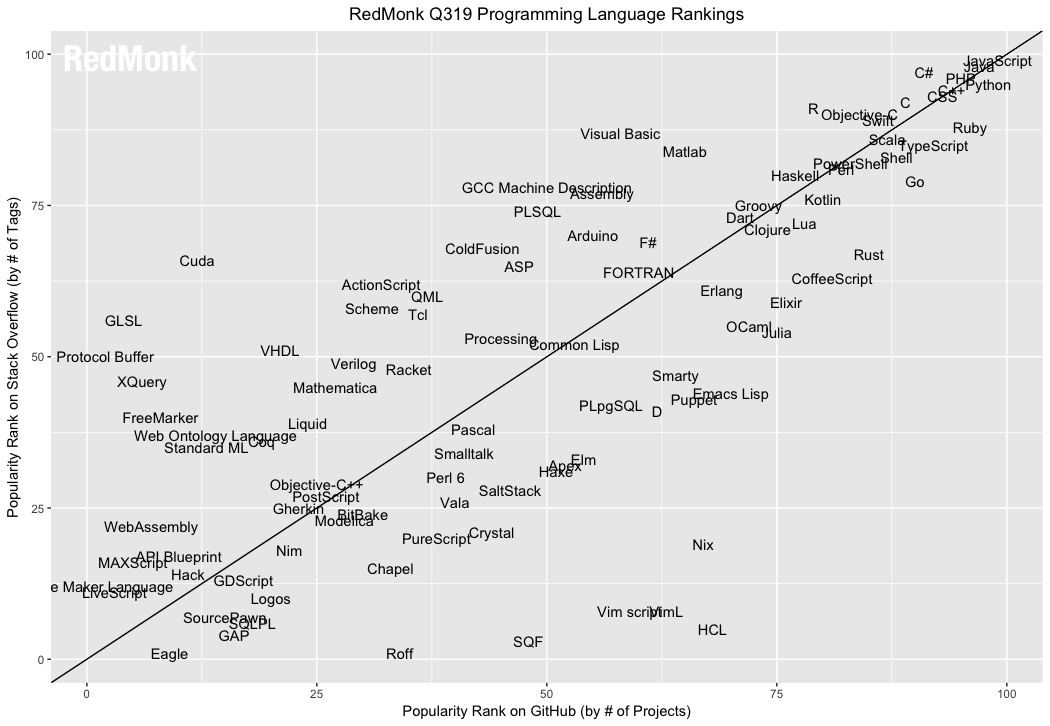
\includegraphics[width=11cm]{c1_intro_language_rank_2019.png}
  \end{figure}
\end{frame}

\begin{frame}
  \frametitle{计算机科学 | 编程语言 | 排名 | 2019}
  \begin{figure}
    \centering
    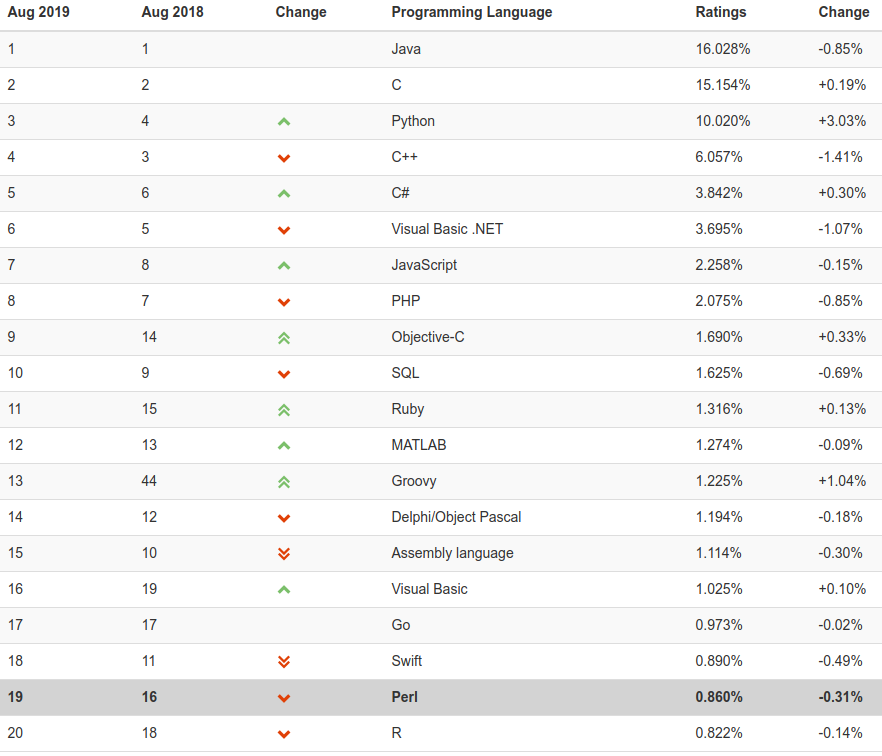
\includegraphics[width=9cm]{c1_intro_language_rate_2019.png}
  \end{figure}
\end{frame}

% \begin{frame}
%   \frametitle{计算机科学 | 编程语言 | 排名 | 趋势}
%   \begin{figure}
%     \centering
%     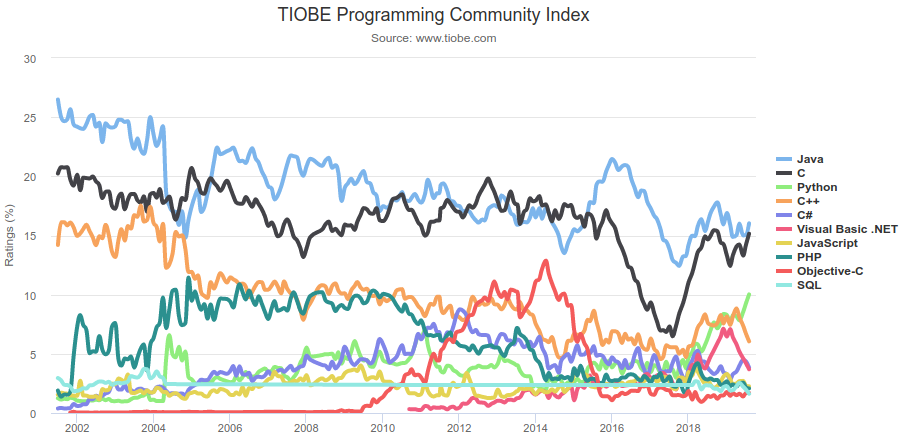
\includegraphics[width=12cm]{c1_intro_language_rate_period_2019.png}
%   \end{figure}
% \end{frame}

\begin{frame}
  \frametitle{计算机科学 | 编程语言 | 排名 | 历史}
  \begin{figure}
    \centering
    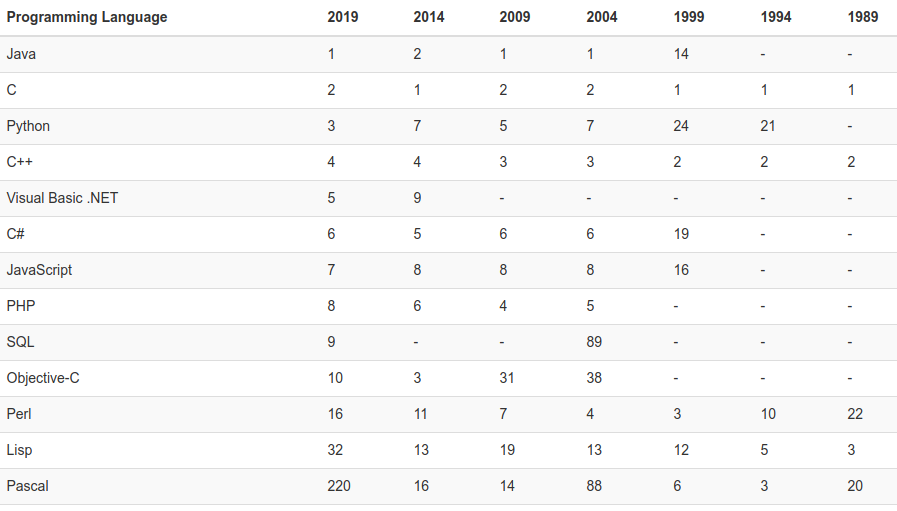
\includegraphics[width=11cm]{c1_intro_language_rate_history_2019.png}
  \end{figure}
\end{frame}

\begin{frame}
  \frametitle{计算机科学 | 编程语言 | 生物信息学}
  \begin{figure}
    \centering
    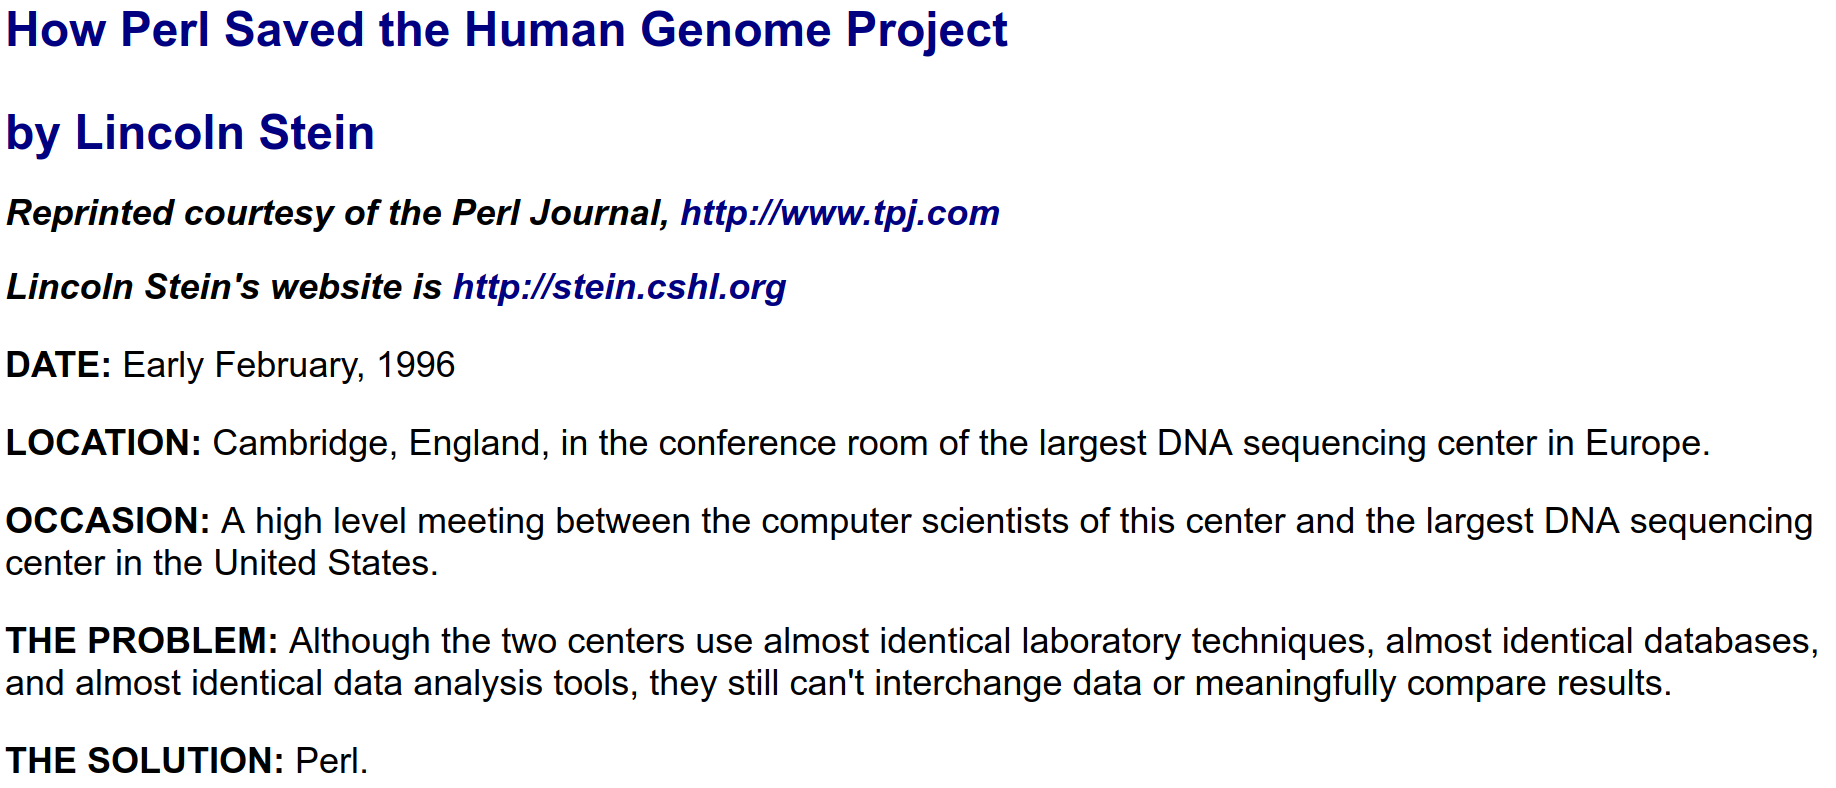
\includegraphics[width=0.9\textwidth]{c1_intro_perl_bx1.png}
  \end{figure}
  \begin{flushright}
    \href{https://web.stanford.edu/class/gene211/handouts/How_Perl_HGP.html}{How Perl Saved the Human Genome Project}
  \end{flushright}
  \begin{quotation}
Perl and the human genome are almost perfectly matched; both are almost incomprehensible, with no central design, accreted haphazardly over a long time.
  \end{quotation}
\end{frame}

\begin{frame}
  \frametitle{计算机科学 | 编程语言 | 生物信息学}
  \begin{block}{\alert{生物信息学常用编程语言}}
    Perl(1987)、Python(1991)、Ruby(1995)、Java(1995)
  \end{block}
  \begin{figure}
    \centering
    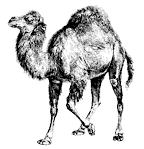
\includegraphics[width=2.5cm]{c1_intro_perl_logo.png}
    \hspace{2em}
    
\includegraphics[width=5.5cm]{c1_intro_python_logo.png}\\
    
\includegraphics[width=2cm]{c1_intro_ruby_logo.png}
    \hspace{11em}
    
\includegraphics[width=1.5cm]{c1_intro_java_logo.png}
  \end{figure}
\end{frame}

\begin{frame}
  \frametitle{计算机科学 | 编程语言 | BioX}
  \begin{block}{\alert{生物信息学专用}}
    BioPerl、Biopython、BioRuby、BioJava
  \end{block}
  \begin{figure}
    \centering
    
\includegraphics[width=2.5cm]{c1_intro_bioperl_logo.png}
    \hspace{2em}
    
\includegraphics[width=6cm]{c1_intro_biopython_logo.jpg}\\
    
\includegraphics[width=2cm]{c1_intro_bioruby_logo.png}
    \hspace{10em}
    
\includegraphics[width=3cm]{c1_intro_biojava_logo.jpg}
  \end{figure}
\end{frame}

% \begin{frame}
%   \frametitle{计算机科学 | 编程语言 | BioSQL}
%   \begin{block}{BioSQL}
%     BioSQL is a generic relational model covering sequences, features, sequence and feature annotation, a reference taxonomy, and ontologies (or controlled vocabularies).\\
%     \vspace{0.3em}
%     Each Bio* project has a language binding (object-relational mapping, ORM) to BioSQL.
%   \end{block}
%   \begin{figure}
%     \centering
%     
\includegraphics[width=0.85\textwidth]{c1_intro_biosql.png}
%   \end{figure}
% \end{frame}

\section{编程}
\begin{frame}
  \frametitle{编程 | 与生物信息学}
  \begin{block}{不需要!}
    \begin{itemize}
      \item 有现成的工具可以使用
      \item 五湖四海皆兄弟
      \item 有钱能使磨推鬼
      \item ……
    \end{itemize}
  \end{block}
  \pause
  \begin{block}{需要!}
    \begin{itemize}
      \item 没有现成的工具
      \item 兄弟们都在忙着混江湖
      \item 工资涨如龟速,物价飙如赤兔
      \item ……
    \end{itemize}
  \end{block}
\end{frame}

\begin{frame}
  \frametitle{编程 | 值得学习 | 现实需求}
  \begin{itemize}
    \item 有助于理解现有工具的配置与个性化修改
    \item 编写程序来批量运行现有程序
    \item 数据分析很简单,前期数据处理很难难难……(二八定律,80/20法则,帕雷托法则)
    \item 增强研究工作的可重复性
    \item 数据越来越大,时间越来越少
    \item 人生苦短,学习编程
    \item ……
  \end{itemize}
\end{frame}

\begin{frame}
  \frametitle{编程 | 值得学习 | 智力投资}
  编程有助于逻辑思维的锻炼,系统观的形成,以及创造能力和解决问题能力的培养。但这些都是潜移默化的,需要有一个积累的过程。
    \begin{itemize}
      \item 试错力:编程的试错成本比较低,在一次次修复bug的过程中,慢慢地就不怕去试错了
      \item 创造力:编程可以把想象变为现实,不断去创造奇迹
      \item 学习能力:编程独特的操作和思考性,不仅会让编程者爱上学习,还会帮助养成严谨、认真的学习习惯
      \item 逻辑思维:一个人语言组织、领导能力的基础
      \item 科学思维:编程就是用科学的眼光去思考问题、分析问题,更全面地去看待这个世界
      \item ……
    \end{itemize}
\end{frame}

\begin{frame}
  \frametitle{编程 | 值得学习 | \alert{编程思维}}
  \begin{block}{编程思维}
    编程思维(computational thinking)就是“理解问题-找出路径”的思维过程,它由分解、模式识别、抽象、算法四个步骤组成。\\
    \vspace{1em}
通过这四个步骤,一个棘手的复杂问题先被拆解成一系列好解决的小问题;每一个小问题被单独检视、思考,搜索解决方法;然后,聚焦几个重要节点,忽视小细节,形成解决思路;最后,设计步骤,执行——问题解决!\\
\vspace{1em}
通过编程做一个作品的过程,就是自己创造一个事物的过程。最起码首先要在心里大致构造出自己想要的作品模样,然后开始思考第一步该怎么做,第二步该怎么做。
  \end{block}
\end{frame}

\begin{frame}
  \frametitle{编程 | 与艺术}
  \begin{figure}
    \centering
    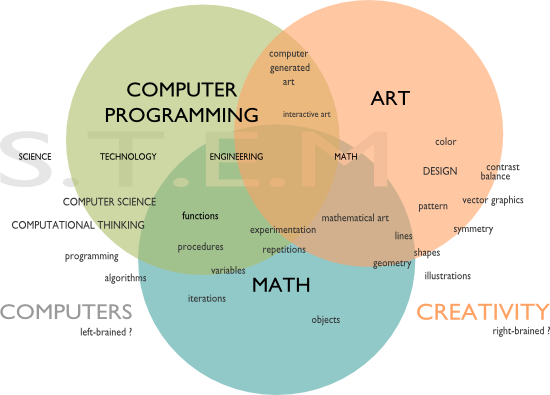
\includegraphics[width=10cm]{c1_intro_programming_art_01.png}
  \end{figure}
\end{frame}

\begin{frame}
  \frametitle{编程 | 与艺术}
  \begin{center}
    \large{每一位程序员都是一位艺术家\\
    每一个程序都是一件艺术品\\
    编写程序 = 艺术创作!}
\end{center}
\vspace{-1em}
  \begin{figure}
    \centering
    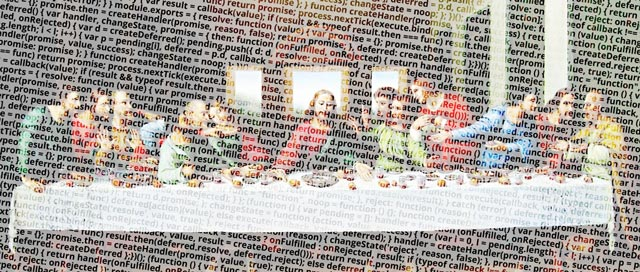
\includegraphics[width=10.5cm]{c1_intro_programming_art_02.jpg}
  \end{figure}
\end{frame}

\begin{frame}
  \frametitle{编程 | 与艺术 | BTW}
  \begin{center}
    \large{If you program enough,\\ it can change the way you look at the world …}
\end{center}
\vspace{-1em}
  \begin{figure}
    \centering
    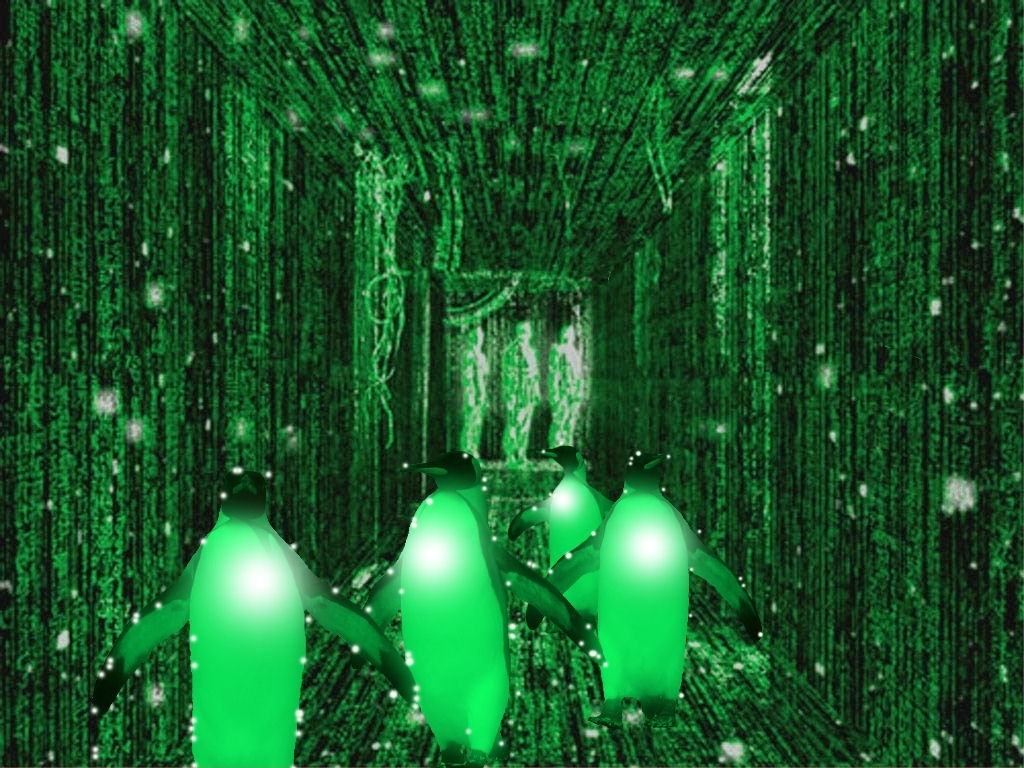
\includegraphics[width=8.5cm]{c1_intro_programming_art_03.jpg}
  \end{figure}
\end{frame}

\begin{frame}
  \frametitle{编程 | 局限 | 理论上无解}
  \begin{block}{任务}
    \begin{enumerate}
      \item<1-> 同时精确测量粒子的位置和动量
      \item<2-> 寻找第四种可以镶嵌平面的凸六边形
      \item<3-> 寻找可以镶嵌平面的边数大于6的凸多边形
      \item<4-> 分析敲除所有必需基因后的基因表达
    \end{enumerate}
  \end{block}
  \begin{block}{原理}
    \begin{enumerate}
      \item<1-> 海森堡不确定性原理
      \item<2-> 有且只有三种凸六边形可以镶嵌平面
      \item<3-> 边数大于6的凸多边形都无法镶嵌平面
      \item<4-> 都说了是必需基因……
    \end{enumerate}
  \end{block}
\end{frame}

\begin{frame}
  \frametitle{编程 | 局限 | (现阶段)实际上不可解}
  \begin{block}{任务}
    \begin{enumerate}
      \item<1-> 破解RSA秘钥
      \item<2-> 暴力破解由94个字符(26小写、26大写、10数字、32标点)随机组合成的长12个字符的密码
      \item<3-> 蛋白质折叠中通过随机尝试找到总能量最低的构象状态
    \end{enumerate}
  \end{block}
  \begin{block}{原因}
    \begin{enumerate}
      \item<1-> 对极大整数做因数分解非常困难(破解RSA-2048(2048-bit)的密钥可能需要耗费传统电脑10亿年的时间,而量子计算机只需要100秒就可以完成。)【量子计算机+秀尔算法】/【黎曼猜想】
      \item<2-> 普通台式机,每秒运算40亿次,需要大约30万年以上才能破解
      \item<3-> 利文索尔佯谬(Levinthal's paradox):100氨基酸,每个2种构象,每次尝试耗时$10^{-13}$s,穷举需要40亿年【深度学习?】
    \end{enumerate}
  \end{block}
\end{frame}

\section{Bioinformatics Career Survey 2008}
\begin{frame}
  \frametitle{2008 | happiness}
   \begin{figure}
     \centering
     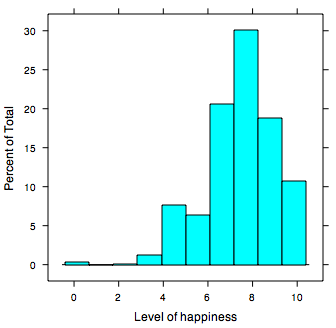
\includegraphics[width=0.65\textwidth]{c1_intro_2008_happiness.png}
   \end{figure}
\end{frame}

\begin{frame}
  \frametitle{2008 | happiness vs. career position}
   \begin{figure}
     \centering
     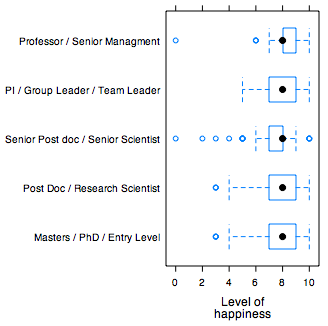
\includegraphics[width=0.65\textwidth]{c1_intro_2008_happiness_position.png}
   \end{figure}
\end{frame}

\begin{frame}
  \frametitle{2008 | likes vs. dislikes}
   \begin{figure}
     \centering
     \includegraphics[width=0.9\textwidth]{c1_intro_2008_happiness_like.png}
   \end{figure}
\end{frame}

\begin{frame}
  \frametitle{2008 | research area}
   \begin{figure}
     \centering
     \includegraphics[width=0.65\textwidth]{c1_intro_2008_area.png}
   \end{figure}
\end{frame}

\begin{frame}
  \frametitle{2008 | research area | clustering}
   \begin{figure}
     \centering
     \includegraphics[width=0.55\textwidth]{c1_intro_2008_area_cluster.png}
   \end{figure}
\end{frame}

\begin{frame}
  \frametitle{2008 | background}
   \begin{figure}
     \centering
     \includegraphics[width=0.7\textwidth]{c1_intro_2008_background.png}
   \end{figure}
\end{frame}

\begin{frame}
  \frametitle{2008 | language}
   \begin{figure}
     \centering
     \includegraphics[width=0.9\textwidth]{c1_intro_2008_language.png}
   \end{figure}
\end{frame}

\begin{frame}
  \frametitle{2012 | language}
   \begin{figure}
     \centering
     \includegraphics[width=0.95\textwidth]{c1_intro_2012_language.png}
   \end{figure}
\end{frame}

\begin{frame}
  \frametitle{Bioinformatics.org (2007) | language}
   \begin{figure}
     \centering
     \includegraphics[width=0.23\textwidth]{c1_intro_language_bx_vote.png}
   \end{figure}
\end{frame}


\begin{frame}
  \frametitle{2008 | applications}
   \begin{figure}
     \centering
     \includegraphics[width=0.53\textwidth]{c1_intro_2008_application.png}
   \end{figure}
\end{frame}

\begin{frame}
  \frametitle{2008 | tools}
   \begin{figure}
     \centering
     \includegraphics[width=0.55\textwidth]{c1_intro_2008_tool.png}
   \end{figure}
\end{frame}

\begin{frame}
  \frametitle{2008 | salary}
  \begin{block}{industry vs. academic}
    \begin{itemize}
      \item Academic Salary Mean/Median: \$36,520 / \$33,712
      \item Industry Salary Mean/Median: \$66,239 / \$64,235
    \end{itemize}
  \end{block}
  \pause
  \begin{block}{Salary/Years Experience}
    \begin{itemize}
      \item Academic Mean/Median: \$10,970 / \$8,333
      \item Industry Mean/Median: \$17,410 / \$12,000
    \end{itemize}
  \end{block}
\end{frame}

\begin{frame}
  \frametitle{2008 | 参考资料}
  \begin{itemize}
    \item \href{http://openwetware.org/wiki/Biogang:Projects/Nioinformatics\_Career\_Survey\_2008}{Bioinformatics Career Survey 2008}
    \item \href{http://openwetware.org/wiki/Biogang:Projects/Bioinformatics\_Career\_Survey\_2008\_Results}{Bioinformatics Career Survey 2008 Results}
    \item \href{https://github.com/michaelbarton/bioinformatics-career-survey}{bioinformatics-career-survey (GitHub)}
    \item \href{http://www.ncbi.nlm.nih.gov/pmc/articles/PMC2267699/}{A comparison of common programming languages used in bioinformatics}
    \item \href{http://www.molecularecologist.com/2012/11/a-comparison-of-bioinformatics-programming-languages/}{A comparison of bioinformatics programming languages}
    \item \href{https://nlcb.wordpress.com/2013/02/23/programming-languages-of-bioinformatics-2/}{Programming Languages of Bioinformatics}
    \item \href{https://www.ncbi.nlm.nih.gov/pubmed/28968751}{A global perspective on evolving bioinformatics and data science training needs}
  \end{itemize}
\end{frame}

\begin{frame}
  \frametitle{Career outlook}
  \begin{block}{\href{https://bioinformaticshome.com/blog/jobs_landscape_2018_2020.html}{\textcolor{white}{Data and Bioinformatics Scientists (2018-26)}}}
    \begin{itemize}
      \item The Future of Jobs
        \begin{itemize}
          \item The top ten job winners
          \item The top ten job losers
        \end{itemize}
      \item What is the career outlook for Bioinformatics (2018-2026)?
        \begin{itemize}
          \item What skills a successful bioinformatician need to have?
          \item Specialization within a branch of bioinformatics is essential
          \item Not all bioinformatics jobs and bioinformatics scientists are the same
          \item Job growth and median wages
          \item Keep an eye on rapid technology development
          \item What technology knowledge employers demand today?
        \end{itemize}
      \item Formal bioinformatics education
      \item Pros and cons of bioinformatics as an interdisciplinary field
    \end{itemize}
  \end{block}
\end{frame}

\section{R}
\begin{frame}
  \frametitle{R | 简介}
  \begin{block}{R}
 R is a free software environment for statistical computing and graphics. It compiles and runs on a wide variety of UNIX platforms, Windows and MacOS.\\
\vspace{0.3em}
\alert{R语言},一种自由软体程式语言与操作环境,主要用于\alert{统计分析、绘图、数据挖掘}。R本来是由来自新西兰奥克兰大学的罗斯·伊哈卡和罗伯特·杰特曼开发(也因此称为R),现在由“R开发核心团队”负责开发。\\
\begin{itemize}
  \item R内建多种统计学及数字分析功能。R的功能也可以透过安装套件(Packages,用户撰写的功能)增强。
  \item R的另一强项是绘图功能,制图具有印刷的素质,也可加入数学符号。
  \item 虽然R主要用于统计分析或者开发统计相关的软体,但也有人用作矩阵计算。其分析速度可媲美专用于矩阵计算的自由软件GNU Octave和商业软件MATLAB。
\end{itemize}
  \end{block}
\end{frame}

\begin{frame}
  \frametitle{R | Packages}
  \begin{block}{Packages}
R的功能能够透过由用户撰写的套件增强。增加的功能有特殊的统计技术、绘图功能,以及编程介面和数据输出/输入功能。这些软件包是由R语言、LaTeX、Java及最常用C语言和Fortran撰写。
  \end{block}
  \pause
  \begin{block}{\alert{CRAN}}
    CRAN为Comprehensive R Archive Network(R综合典藏网)的简称。它除了收藏了R的执行档下载版、原始码和说明文件,也收录了各种用户撰写的软件包。现时,全球有超过一百个CRAN镜像站。
  \end{block}
  \pause
  \begin{block}{\alert{Bioconductor}}
    生物信息学社群时常使用R进行分子生物学数据分析。Bioconductor计划就是让R作为基因图谱分析工具。
  \end{block}
\end{frame}

\begin{frame}
  \frametitle{R | IDE}
  \begin{block}{\alert{RStudio}}
 RStudio is an integrated development environment (IDE) for R. It includes a console, syntax-highlighting editor that supports direct code execution, as well as tools for plotting, history, debugging and workspace management.\\
 \vspace{0.3em}
 RStudio is available in open source and commercial editions and runs on the desktop (Windows, Mac, and Linux) or in a browser connected to RStudio Server or RStudio Server Pro (Debian/Ubuntu, RedHat/CentOS, and SUSE Linux).
  \end{block}
  \pause
  \begin{block}{RCode}
    A modern environment for R.
  \end{block}
\end{frame}

\begin{frame}
  \frametitle{R | Packages}
  \begin{block}{Useful and popular packages: Load data}
    \begin{description}
      \item[\alert{readr}] readr makes it easy to read many types of \alert{tabular data} including: delimited files, fixed width files and web log files.
      \item[\alert{readxl}] Import \alert{excel files} into R. readxl supports both the legacy .xls format and the modern xml-based .xlsx format.
      \item[XLConnect] Help you read, write and format \textbf{Micorsoft Excel} files from R.
      \item[foreign] Functions for reading and writing data stored by some versions of Epi Info, Minitab, S, SAS, SPSS, Stata, Systat and Weka and for reading and writing some dBase files.
      \item[httr] A set of useful tools for working with \textbf{http} connections.
      \item[XML] Read and create \textbf{XML} documents with R.
      \item[jsonlite] Read and create \textbf{JSON} data tables with R.
    \end{description}
  \end{block}
\end{frame}

\begin{frame}[fragile]
  \frametitle{R | Packages}
  \begin{block}{Useful and popular packages: Manipulate data}
    \begin{description}
      \item[\alert{tidyr}] Tools for changing the layout of your data sets. Use the gather and spread functions to convert your data into the \alert{tidy format}, the layout R likes best.
      \item[\alert{magrittr}] magrittr provides a mechanism for chaining commands with a new \alert{forward-pipe operator}, \verb|%>%|.
      \item[\alert{dplyr}] Essential shortcuts for subsetting, summarizing, rearranging, and joining together data sets for \alert{fast data manipulation}.
    \end{description}
  \end{block}
\end{frame}

\begin{frame}[fragile]
  \frametitle{R | Packages}
  \begin{block}{Useful and popular packages: Manipulate data}
    \begin{description}
      \item[\alert{lubridate}] Tools that make working with \alert{dates and times} easier.
      \item[\alert{stringr}] Easy to learn tools for \alert{regular expressions and character strings}.
      \item[plyr] plyr is a set of tools for a common set of problems: you need to \textbf{split} up a big data structure into homogeneous pieces, \textbf{apply} a function to each piece and then \textbf{combine} all the results back together.
      \item[DT] The R package DT provides an R interface to the JavaScript library DataTables. R data objects (matrices or data frames) can be displayed as tables on HTML pages, and DataTables provides filtering, pagination, sorting, and many other features in the tables.
    \end{description}
  \end{block}
\end{frame}

\begin{frame}
  \frametitle{R | Packages}
  \begin{block}{Useful and popular packages: Visualize data}
    \begin{description}
      \item[\alert{ggplot2}] R's famous package for making beautiful graphics. ggplot2 lets you use \alert{the grammar of graphics} to build layered, customizable plots.
      \item[ggvis] \textbf{Interactive, web based graphics} built with the grammar of graphics.
      \item[DiagrammeR] Create \textbf{graph diagrams and flowcharts} using R.
      \item[htmlwidgets] The htmlwidgets package provides a framework for easily creating R bindings to JavaScript libraries.
    \end{description}
  \end{block}
\end{frame}

\begin{frame}
  \frametitle{R | Packages}
  \begin{block}{Useful and popular packages: Report results}
    \begin{description}
      \item[\alert{rmarkdown}] rmarkdown lets you insert R code into a \alert{markdown document}. R then generates a final document, in a wide variety of formats, that replaces the R code with its results.
      \item[\alert{knitr}] knitr is an elegant, flexible and fast dynamic report generation that combines R with TeX, Markdown, or HTML. For open access publishing, and \alert{reproducible research} in statistics.
      \item[\alert{xtable}] The xtable function takes an R object (like a data frame) and returns the latex or HTML code you need to paste a pretty version of the object into your documents. Copy and paste, or pair up with R Markdown.
    \end{description}
  \end{block}
\end{frame}

\begin{frame}
  \frametitle{R | Packages}
  \begin{block}{Useful and popular packages: Report results}
    \begin{description}
      \item[Shiny] Easily make \textbf{interactive, web apps} with R. A perfect way to explore data and share findings with non-programmers.
      \item[shinydashboard] shinydashboard makes it easy to use Shiny to create dashboards.
    \end{description}
  \end{block}
\end{frame}

\begin{frame}
  \frametitle{R | Packages}
  \begin{block}{Useful and popular packages: High performance}
    \begin{description}
      \item[\alert{data.table}] An alternative way to organize data sets for \alert{very, very fast} operations. Useful for big data.
      \item[parallel] Use \textbf{parallel processing} in R to speed up your code or to crunch large data sets.
      \item[\alert{foreach}] Provides Foreach Looping Construct for R. Foreach is an idiom that allows for iterating over elements in a collection, without the use of an explicit loop counter. Using foreach without side effects also facilitates \textbf{executing the loop in parallel}.
      \item[\alert{doParallel}] Foreach Parallel Adaptor for the `parallel' Package. Provides a parallel backend for the \textbf{\%dopar\%} function using the parallel package.
    \end{description}
  \end{block}
\end{frame}

\begin{frame}
  \frametitle{R | Packages}
  \begin{block}{Useful and popular packages: Development}
    \begin{description}
      \item[devtools] An essential suite of tools for turning your code into an R package.
      \item[roxygen2] A quick way to \textbf{document} your R packages. roxygen2 turns inline code comments into documentation pages and builds a package namespace.
      \item[testthat] testthat provides an easy way to write \textbf{unit tests} for your code projects.
    \end{description}
  \end{block}
\end{frame}

\begin{frame}
  \frametitle{R | Packages}
  \begin{block}{Easily install and load packages from the tidyverse}
    The \alert{tidyverse} is a collection of R packages that share common philosophies and are designed to work together.\\
    \vspace{0.3em}
    The \alert{core tidyverse packages} that you are likely to use in almost every analysis:
    \begin{itemize}
      \item readr, for data import.
      \item tidyr, for data tidying.
      \item dplyr, for data manipulations.
      \item ggplot2, for data visualisation.
      \item stringr, for string manipulations.
      \item purrr, for functional programming.
      \item tibble, for tibbles, a modern re-imagining of data frames.
      \item forcats, a suite of useful tools that solve common problems with factors.
    \end{itemize}
  \end{block}
\end{frame}

\begin{frame}[fragile]
  \frametitle{R | Packages}
  \begin{block}{Easily install and load packages from the tidyverse}
    It also installs a selection of other tidyverse packages that you're likely to use frequently, but probably not in every analysis. This includes packages for:
    \begin{itemize}
      \item Working with specific types of vectors: hms (times), stringr (strings), lubridate (date/times), forcats (factors), blob (blob/binary data).
      \item Importing other types of data: DBI (databases), haven (SPSS, SAS and Stata files), httr (web apis), jsonlite (JSON), readxl (.xls and .xlsx files), rvest (web scraping), xml2 (XML).
      \item Programming and modelling: magrittr (\verb|%>%|), glue (alternative to paste()), modelr (modelling within a pipeline), broom (turning models into tidy data).
    \end{itemize}
  \end{block}
\end{frame}

\begin{frame}[fragile]
  \frametitle{R | Packages}
  \begin{block}{Others}
    \begin{description}
      \item[\alert{swirl}] Learn R, in R
      \item[learnr] Interactive Tutorials for R
      \item[officer] Manipulation of Microsoft Word and PowerPoint Documents
      \item[export] Streamlined Export of Graphs and Data Tables
      \item[\alert{argparse}] A command line parser to be used with Rscript to write \verb|"#!"| shebang scripts that gracefully accept positional and optional \alert{arguments} and automatically generate usage.
    \end{description}
  \end{block}
\end{frame}

\begin{frame}[fragile]
  \frametitle{R | Packages}
  \begin{block}{Others}
    \begin{description}
      \item[viridis] Use the color scales in this package to make plots that are pretty, better represent your data, easier to read by those with colorblindness, and print well in grey scale. 
      \item[ggthemes] Extra Themes, Scales and Geoms for `ggplot2'
      \item[\alert{ggsci}] Scientific Journal and Sci-Fi Themed Color Palettes for `ggplot2'
      \item[\alert{ggpubr}] `ggplot2' Based Publication Ready Plots
      \item[ggthemr] Themes for ggplot2
      \item[ggtech] ggplot2 tech themes, scales, and geoms
      \item[bbplot] R package that helps create and export ggplot2 charts in the style used by the BBC News data team
    \end{description}
  \end{block}
\end{frame}

\begin{frame}[fragile]
  \frametitle{R | Packages}
  \begin{block}{Others}
    \begin{description}
      \item[\alert{ggtree}] Visualization and annotation of \alert{phylogenetic trees}.
      \item[\alert{ComplexHeatmap}] ComplexHeatmap package provides a highly flexible way to arrange multiple \alert{heatmaps} and supports self-defined annotation graphics. 
      \item[esquisse] Explore and Visualize Your Data Interactively
      \item[rattle] Graphical User Interface for Data Science in R
      \item[visreg] Visualization of Regression Models
      \item[ggThemeAssist] Add-in to Customize `ggplot2' Themes
      \item[ggedit] Interactive 'ggplot2' Layer and Theme Aesthetic Editor
      \item[gganimate] A Grammar of Animated Graphics
    \end{description}
  \end{block}
\end{frame}

\begin{frame}
  \frametitle{R | \alert{Bioconductor}}
  \begin{block}{Bioconductor}
    Bioconductor provides tools for the analysis and comprehension of high-throughput genomic data. Bioconductor uses the R statistical programming language, and is open source and open development.
  \end{block}
  \begin{figure}
    \centering
    \includegraphics[width=0.9\textwidth]{c1_intro_bioconductor_logo.jpg}
  \end{figure}
\end{frame}

\begin{frame}[fragile]
  \frametitle{R | Example}
\begin{lstlisting}[language=R]
# 下页幻灯片(左上角)第一个图
n <- 50000
r <- 0.7
r_e <- (1 - r * r) ^ 0.5
X <- rnorm(n)
Y <- X * r + r_e * rnorm(n)
Y <- ifelse(X>0, Y, -Y)
plot(X, Y, col="pink")
\end{lstlisting}
\end{frame}

\begin{frame}
  \frametitle{R | Example}
  \begin{figure}
    \centering
    \includegraphics[width=0.35\textwidth]{c1_r_plot_01.png}\qquad
    \includegraphics[width=0.4\textwidth]{c1_r_plot_03.png}\\
    \includegraphics[width=0.3\textwidth]{c1_r_plot_02.png}
    \hspace{4em}
    \includegraphics[width=0.25\textwidth]{c1_r_plot_04.png}
  \end{figure}
\end{frame}

\begin{frame}[fragile]
  \frametitle{R | Example | Female body}
  \vspace{-1.5em}
\begin{lstlisting}[language=R,basicstyle=\footnotesize\tt]
xrange <- c(-15, 15); yrange <- c(0, 16)
plot(0, xlim=xrange, ylim=yrange, type="n")

yr <- seq(yrange[1], yrange[2], len=50)
offsetFn <- function(y) { 2 * sin(0 + y/3) }
offset <- offsetFn(yr)
leftE <- function(y) { -10 - offsetFn(y) }
rightE <- function(y) { 10 + offsetFn(y) }
xp <- c(leftE(yr), rev(rightE(yr)))
yp <- c(yr, rev(yr))
polygon(xp, yp, col="#ffeecc", border=NA)

h <- 9
xt <- seq(0, rightE(h), len=100)
yt <- log(1 + log(1 + log(xt + 1)))
yt <- yt - min(yt); yt <- h * yt/max(yt)
x <- c(leftE(h), rightE(h), rev(xt), -xt)
y <- c(h, h, rev(yt), yt)
polygon(x, y, col="red", border=NA)
\end{lstlisting}
\end{frame}

\begin{frame}
  \frametitle{R | Example}
  \begin{figure}
    \centering
    \includegraphics[width=0.9\textwidth]{c1_r_gapminder_2016.png}
  \end{figure}
\end{frame}

\begin{frame}[fragile]
  \frametitle{R | Example | parallel}
\begin{lstlisting}[language=R]
#!/usr/bin/Rscript

# print 1 to 10: use 20 seconds
system.time(
  for (i in 1:10) {
    Sys.sleep(2)
    print(i)
  }
)
\end{lstlisting}
\end{frame}

\begin{frame}[fragile]
  \frametitle{R | Example | parallel}
  \vspace{-0.5em}
\begin{lstlisting}[language=R]
#!/usr/bin/Rscript
library(foreach)
library(doParallel)

# no_cores <- detechCores() - 1
no_cores <- 10
cl <- makeCluster(no_cores)
registerDoParallel(cl)

system.time(
  x <- foreach (i=1:10) %dopar% {
    Sys.sleep(2); print(i)
  }
)

stopCluster(cl)
\end{lstlisting}
\end{frame}

\begin{frame}
  \frametitle{R | 参考资料}
   \begin{itemize}
     \item \href{https://www.r-project.org/}{The R Project for Statistical Computing}
     \item \href{https://www.rstudio.com/}{RStudio}
     \item \href{https://support.rstudio.com/hc/en-us/categories/200098757-Learn-R}{Learn R}
     \item \href{https://www.rstudio.com/resources/cheatsheets/}{RStudio Cheat Sheets}
     \item \href{https://www.rstudio.com/products/rpackages/}{R packages inspired by R and its community}
     \item \href{https://support.rstudio.com/hc/en-us/articles/201057987-Quick-list-of-useful-R-packages}{Quick list of useful R packages}
     \item \href{https://www.bioconductor.org/}{Bioconductor}
   \end{itemize}
\end{frame}

\section{书籍}
\begin{frame}
  \frametitle{书籍 | Perl}
  \begin{block}{生物信息学角度}
    \textit{\alert{Beginning}} $\Longrightarrow$ \textit{Mastering Perl for Bioinformatics}
  \end{block}
  \begin{figure}
    \centering
    \includegraphics[width=4.5cm]{c2_perl_bpfb.jpg}
    \hspace{1em}
    \includegraphics[width=4.5cm]{c2_perl_mpfb.jpg}
  \end{figure}
\end{frame}

\begin{frame}
  \frametitle{书籍 | Perl}
  \begin{block}{编程语言角度:代号}
小骆驼 $\Rightarrow$ 羊驼书 $\Rightarrow$ 小羊驼母亲和她的孩子 $\Rightarrow$ 大骆驼 $\Rightarrow$ 黑豹书
  \end{block}
  \pause
  \begin{block}{英文名}
    \textit{Learning Perl} $\Rightarrow$ \textit{Intermediate Perl} $\Rightarrow$ \textit{Mastering Perl} $\Rightarrow$ \textit{Programming Perl} $\Rightarrow$ \textit{Advanced Perl Programming}
  \end{block}
  \pause
  \begin{block}{中文名}
    \alert{《Perl语言入门》} $\Rightarrow$ 《Perl进阶》 $\Rightarrow$ 《精通Perl》 $\Rightarrow$ 《Perl语言编程》 $\Rightarrow$ 《高级Perl编程》
  \end{block}
  \pause
\end{frame}

\begin{frame}
  \frametitle{书籍 | Perl}
  \begin{figure}
    \centering
    \includegraphics[width=3cm]{c2_perl_lp.png}
    \qquad
    \includegraphics[width=3cm]{c2_perl_ip.png}
    \qquad
    \includegraphics[width=3cm]{c2_perl_mp.jpg}\\
    \includegraphics[width=3cm]{c2_perl_pp.png}
    \hspace{2cm}
    \includegraphics[width=3cm]{c2_perl_app.jpg}
  \end{figure}
\end{frame}

\begin{frame}
  \frametitle{书籍 | Perl}
  \begin{columns}
    \column{0.4\textwidth}
  \begin{block}{中文名}
    \begin{itemize}
      \item \alert{《Perl入门经典》}
      \item 《高阶Perl》
      \item 《Perl高效编程》
      \item 《Perl最佳实践》
      \item \textit{Perl Cookbook}
    \end{itemize}
  \end{block}
    \column{0.5\textwidth}
  \begin{block}{英文名}
    \begin{itemize}
      \item \textit{Beginning Perl}
      \item \textit{Higher-Order Perl}
      \item \textit{Effective Perl Programming}
      \item \textit{Perl Best Practices}
      \item \textit{Perl Cookbook}
    \end{itemize}
  \end{block}
\end{columns}
\end{frame}

\begin{frame}
  \frametitle{书籍 | Perl}
  \begin{figure}
    \centering
    \includegraphics[height=3.8cm]{c1_book_perl_bp.jpg}\qquad
    \includegraphics[height=3.8cm]{c1_book_perl_hop.jpg}\\
    \includegraphics[height=3.85cm]{c1_book_perl_epp.jpg}\quad
    \includegraphics[height=3.85cm]{c1_book_perl_pbp.jpg}\quad
    \includegraphics[height=3.85cm]{c1_book_perl_pc.png}
  \end{figure}
\end{frame}

\begin{frame}
  \frametitle{书籍 | Python}
  \begin{columns}
    \column{0.4\textwidth}
  \begin{block}{中文名}
    \begin{itemize}
      \item 《趣学Python编程》
      \item 《父与子的编程之旅:与小卡特一起学Python 》
      \item 《Python学习手册》
      \item 《深入浅出Python》
      \item 《“笨办法”学Python》
      \item 《像计算机科学家一样思考Python》
      \item \textit{Python Cookbook}
    \end{itemize}
  \end{block}
    \column{0.55\textwidth}
  \begin{block}{英文名}
    \begin{itemize}
      \item \textit{Python for Kids}
      \item \textit{Computer Programming for Kids and Other Beginners}
      \item \textit{Learning Python}
      \item \textit{Head First Python}
      \item \textit{Learn Python the Hard Way}
      \item \textit{Think Python}
        \vspace{1em}
      \item \textit{Python Cookbook}
    \end{itemize}
  \end{block}
\end{columns}
\end{frame}

\begin{frame}
  \frametitle{书籍 | Python}
  \begin{figure}
    \centering
    \includegraphics[height=3.5cm]{c1_book_python_pfk.jpg}\quad
    \includegraphics[height=3.5cm]{c1_book_python_cpk.jpg}\quad
    \includegraphics[height=3.5cm]{c1_book_python_lp.jpg}\\
    \includegraphics[height=3.3cm]{c1_book_python_hfp.jpg}\quad
    \includegraphics[height=3.3cm]{c1_book_python_lphw.jpg}\quad
    \includegraphics[height=3.3cm]{c1_book_python_tp.jpg}\quad
    \includegraphics[height=3.3cm]{c1_book_python_pc.jpg}
  \end{figure}
\end{frame}

\begin{frame}
  \frametitle{书籍 | R}
  \begin{columns}
    \column{0.4\textwidth}
  \begin{block}{中文名}
    \begin{itemize}
      \item \alert{《学习R》}
      \item 《R语言初学指南》
      \item 《R语言实战》
      \item \alert{《R语言经典实例》}
      \item \alert{《R数据可视化手册》}
      \item \alert{《R数据科学》}
    \end{itemize}
  \end{block}
    \column{0.5\textwidth}
  \begin{block}{英文名}
    \begin{itemize}
      \item \textit{Learning R}
      \item \textit{The R Student Companion}
      \item \textit{R in Action}
      \item \textit{R Cookbook}
      \item \textit{R Graphics Cookbook}
      \item \textit{R for Data Science}
    \end{itemize}
  \end{block}
\end{columns}
\end{frame}

\begin{frame}
  \frametitle{书籍 | R}
  \begin{figure}
    \centering
    \includegraphics[height=3.8cm]{c1_book_r_lr.jpg}\qquad
    \includegraphics[height=3.8cm]{c1_book_r_trsc.jpg}\qquad
    \includegraphics[height=3.8cm]{c1_book_r_ria.jpg}\\
    \includegraphics[height=3.8cm]{c1_book_r_rc.jpg}\qquad
    \includegraphics[height=3.8cm]{c1_book_r_rgc.jpg}\qquad
    \includegraphics[height=3.8cm]{c1_book_r_rfds.png}\\
  \end{figure}
\end{frame}

\begin{frame}
  \frametitle{书籍 | Python与R | 补遗}
  \begin{itemize}
    \item 《Python数据科学手册》
    \item 《Python数据科学入门》
    \item 《Python数据分析基础》
    \item 《Python编程入门》
    \item 《Python基础教程》
    \item 《Python语言及其应用》
    \item 《Python编程——从入门到实践》
    \item 《R语言入门与实践》
    \item 《R语言:从数据思维到数据实战》
    \item 《R语言数据可视化之美:专业图表绘制指南》
  \end{itemize}
\end{frame}

\begin{frame}
  \frametitle{书籍 | 其他}
  \begin{block}{计算机科学与程序设计}
    \begin{columns}
        \column{0.4\textwidth}
    \begin{itemize}
      \item \alert{《Linux Shell脚本攻略》}
      \item 《我的第一本编程书》
      \item 《教孩子学编程》
      \item 《编程导论》
      \item 《深入浅出程序设计》
      \item 《程序是怎样跑起来的》
      \item 《写给大家看的算法书》
      \item 《啊哈!算法》
      \item 《算法的乐趣》
      \item 《算法帝国》
      \item 《算法笔记》
      \item 《轻松学算法》
    \end{itemize}
        \column{0.6\textwidth}
    \begin{itemize}
      \item 《数据结构与算法图解》
      \item 《大话数据结构》
      \item 《程序员的数学》
      \item 《程序员的数学2:概率统计》
      \item 《程序员的数学3:线性代数》
      \item 《统计思维:程序员数学之概率统计》
      \item 《程序员的数学思维修炼》
    \end{itemize}
  \end{columns}
  \end{block}
\end{frame}

\begin{frame}
  \frametitle{书籍 | 其他}
    \begin{block}{数据科学}
      \begin{itemize}
        \item 《数据科学入门》
        \item 《面向数据科学家的实用统计学》
        \item 《命令行中的数据科学》
        \item 《深入浅出数据分析》
        \item 《菜鸟侦探挑战数据分析》
      \end{itemize}
  \end{block}
\end{frame}

\begin{frame}
  \frametitle{书籍 | 其他}
    \begin{block}{统计学}
    \begin{columns}
        \column{0.5\textwidth}
    \begin{itemize}
      \item 《统计学》(\textit{Statistics for Engineers and the Sciences})
      \item 《统计学及其应用》
      \item 《深入浅出统计学》
      \item 《从零开始学统计》
      \item 《从零开始读懂统计学》
      \item 《白话统计》
      \item 《白话统计学》
      \item 《爱上统计学》
    \end{itemize}
        \column{0.5\textwidth}
    \begin{itemize}
      \item \alert{《赤裸裸的统计学》}
      \item 《你一定爱读的极简统计学》
      \item 《介绍丛书:统计学》
      \item 《漫画玩转统计学》
      \item 《漫画统计学》
    \end{itemize}
  \end{columns}
  \end{block}
\end{frame}

\begin{frame}
  \frametitle{书籍 | 其他}
    \begin{block}{统计学科普}
      \begin{itemize}
      \item 《统计学的世界》
      \item 《统计学漫话》
      \item 《统计学七支柱》
      \item 《数字唬人》
      \item 《统计数字会撒谎》
      \item 《统计数据的真相》
      \item 《生活中的概率趣事》
      \item 《改变世界的134个概率统计故事》
      \item 《统计会犯错——如何避免数据分析中的统计陷阱》
      \item 《妙趣横生的统计学——培养大数据时代的统计思维》
      \item 《别拿相关当因果——因果关系简易入门》
      \end{itemize}
    \end{block}
\end{frame}

\section{回顾与总结}
\subsection{总结}
\begin{frame}
  \frametitle{绪论 | 总结}
  \begin{block}{知识点}
    \begin{itemize}
      \item 生物信息学:交叉学科,多种技能,领域宽泛
      \item 生物学:DNA,RNA,蛋白质
      \item 计算机科学:三个术语,编程语言
      \item R:readr、tidyr、dplyr、ggplot2等常用包
    \end{itemize}
  \end{block}
\end{frame}

\subsection{思考题}
\begin{frame}
  \frametitle{绪论 | 思考题}
  \begin{enumerate}
    \item 生物信息学主要是由哪些学科交叉而来的?
    \item 生物信息学主要需要哪些方面的知识和技能?
    \item DNA是由哪四种碱基组成的?RNA与之有何不同?
    \item 列举常见的20种氨基酸,它们三字母和单字母的缩写分别是什么?
    \item 列举常见的存储DNA序列和蛋白质结构的数据库。
    \item \textit{in vivo}、\textit{in vitro}和\textit{in silico}分别代表什么含义?
    \item 列举常见的编程语言,在生物信息学中常用的编程语言,专用于生物信息学的工具集。
    \item 列举R的常用包并简介其主要用途。
  \end{enumerate}
\end{frame}

\begin{frame}
  \frametitle{下节预告}
  \begin{block}{Markdown}
    回顾、总结Markdown标记语言的基本语法:
    \begin{itemize}
      \item 标题
      \item 强调
      \item 列表
      \item 代码
      \item 引用
      \item 链接
      \item ……
    \end{itemize}
  \end{block}
\end{frame}

\input{snippet/class_tail}
